\chapter{Sistemas dinâmicos}

\section{Definições gerais}

\subsection{Sistemas dinâmicos discretos e contínuos}

\begin{definition}
Um \emph{sistema dinâmico discreto} é uma dupla $(X,f)$ em que
	\begin{enumerate}
	\item $X$ é um conjunto, o \emph{espaço de fase} do sistema;
	\item $\fun{f}{X}{X}$ é uma função, a \emph{dinâmica} do sistema.
	\end{enumerate}
Um sistema dinâmico discreto \emph{invertível} (ou \emph{revertível}) é um sistema dinâmico $(X,f)$ cuja dinâmica $f$ é invertível.
\end{definition}

Além de sistemas dinâmicos discretos, podemos também considerar sistemas dinâmicos contínuos, que são definidos a partir de um semifluxo $f$ no espaço de fase $X$ da forma
	\begin{align*}
	\func{f}{\R_{\geq 0}  \times X}{X}{(t,x)}{f^t(x)},
	\end{align*}
que também pode ser entendido como uma função $\fun{f}{\R_{\geq 0}}{\Func(X,X)}$ que é uma ação do monoide aditivo $\R_{\geq}$ sobre o espaço $X$, ou seja, um homomorfismo de monoides entre o monoide aditivo $\R_{\geq 0}$ e o monoide de composição de funções no espaço de funções $\Func(X,X)$.

\begin{definition}
Um \emph{sistema dinâmico contínuo} é uma dupla $(X,f)$ em que
	\begin{enumerate}
	\item $X$ é um conjunto, o \emph{espaço de fase} do sistema;
	\item $\fun{f}{\R_{\geq 0}  \times X}{X}$ é um semifluxo, a \emph{dinâmica} do sistema.
	\end{enumerate}
\end{definition}

Esse semifluxo pode ser também um fluxo completo, no sentido que de estar definido para todo $\R$, não somente em $\R_{\geq 0}$. Nesse caso, o fluxo seria uma função $\fun{f}{\R  \times X}{X}$, uma ação do grupo aditivo $\R$, o sistema seria \emph{invertível} (ou \emph{revertível}).

Essas duas definições estão relacionadas. No caso de um sistema dinâmico contínuo, podemos considerar o mapa de tempo $1$ do (semi)fluxo, $\fun{f^1}{X}{X}$, que nos dá um sistema dinâmico discreto em $X$. Por outro lado, a partir de um sistema discreto cuja dinâmica é $\fun{f}{X}{X}$, podemos considerar as composições sucessivas da dinâmicas consigo mesma, denotadas $f^n = f \circ \cdots \circ f$, de modo que teríamos uma ação de $\Z_{\geq 0}$ sobre $X$ (ou de $\Z$ caso o sistema seja invertível). Sob essa perspectiva, podemos definir uma noção mais geral de sistema dinâmico.

\begin{definition}
Seja $\bm M$ um monoide. Um \emph{sistema $\bm M$-dinâmico} é um par $(X,f)$ em que
	\begin{enumerate}
	\item $X$ é um conjunto, o \emph{espaço de fase} do sistema;
	\item $f\colon \bm T \age X$ é uma ação de monoides em $X$, a \emph{dinâmica} do sistema.
	\end{enumerate}
\end{definition}

\begin{comment}
\begin{definition}
Um \emph{sistema dinâmico} é uma tripla $\Sist=(X,\bm T,f)$ em que
\begin{enumerate}
\item $X$ é um conjunto, o \emph{espaço de fase} do sistema;
\item $\bm T$ é um monoide, o \emph{espaço temporal} do sistema;
\item $f\colon \bm T \age X$ é uma ação de monoides em $X$, a \emph{dinâmica} do sistema.
\end{enumerate}
\end{definition}
\end{comment}

Por essa definição, sistemas dinâmicos discretos são \emph{sistemas $\Z_{\geq 0}$-dinâmicos} (ou \emph{$\Z$-dinâmicos} no caso invertível) e sistemas dinâmicos contínuos são \emph{sistemas $\R_{\geq 0}$-dinâmicos} (ou \emph{$\R$-dinâmicos} no caso invertível). Pode-se se considerar a ação de monoides e grupos mais gerais --- às vezes $\Z^d$, $\R^d$ ou até algum grupo abstrato --- mas isso não será feito aqui. Estudaremos principalmente sistemas dinâmicos discretos e, ocasionalmente, sistemas contínuos.

\subsection{Órbitas}

A partir de agora, apresentaremos as definições apenas para sistemas dinâmicos discretos.

\begin{definition}[Iterados e conjunto órbita]
Sejam $(X,f)$ um sistema dinâmico discreto, $x \in X$ e $i \in \Z_{\geq 0}$ (ou $i \in \Z$ caso o sistema seja invertível). O \emph{$i$-ésimo iterado de $x$} é o ponto $f^i(x)$.

Seja $I \subseteq \Z_{\geq}$ (ou $I \subseteq \Z$ caso o sistemas seja invertível). O \emph{conjunto de $I$-iterados de $x$} é
	\begin{equation*}
	f^I(x) := \set{f^i(x)}{i \in I}.
	\end{equation*}
O \emph{conjunto órbita} de um ponto $x$ é o conjunto $\Orb(x) := f^{\Z_{\geq 0}}(x)$ (caso o sistema seja invertível, o \emph{conjunto órbita} de $x$ é $\Orb(x) := f^\Z(x)$ e o \emph{conjunto de semiórbita positiva} de $x$ é o conjunto $\Orb^+(x) := f^{\Z_{\geq 0}}(x)$); .
\end{definition}
A mesma definição vale para sistemas contínuos.

%Quando um sistema é irrevertível, cada órbita de um ponto do sistema é igual a sua (semi)órbita positiva. Se o sistema é revertível, pode-se definir a \emph{(semi)órbita negativa} de $x$ como o conjunto $\Orb^-(x) := \set{f^{-t}(x)}{t \in T^+}$, mas não faremos uso dessa estrutura nestas notas.

Na definição anterior, consideramos o conjunto dos iterados de um ponto $x$, ou seja, os ponto pelos quais o ponto $x$ passará ou, no caso invertível, pelos quais ele passou. No entanto, podemos também considerar a órbita como uma sequência de pontos de modo a ter informação sobre em qual tempo o ponto original passou por cada ponto de sua órbita. Consideraremos essa definição a seguir. Para isso, devemos usar sequências de pontos do espaço de fase, isto é, elementos $(x_i)_{i \in \Z}$ de $X^\Z$.

\begin{definition}[Órbitas e espaço de órbitas]
Seja $(X,f)$ um sistema dinâmico discreto. Uma \emph{órbita} de $(X,f)$ é uma sequência $(x_i)_{i \in \Z} \in X^\Z$ tal que, para todo $i \in \Z$, $f(x_i) = x_{i+1}$. O \emph{espaço de órbitas de $(X,f)$} é
	\begin{equation*}
	\orb X := \set{(x_i)_{i \in \Z} \in X^\Z}{\forall_{i \in \Z}\ f(x_i) = x_{i+1}},
	\end{equation*}
o conjunto das órbitas do sistema. A \emph{dinâmica do espaço de órbitas} é a função
	\begin{align*}
	\func{\orb f}{\orb X}{\orb X}{(x_i)_{i \in \Z}}{(f(x_i))_{i \in \Z}.}
	\end{align*}
\end{definition}

Note que, para toda órbita $\widetilde{x} \in \widetilde{X}$, vale $(f(x_i))_{i \in \Z} = (x_{i+1})_{i \in \Z}$, pois por definição de órbita vale $f(x_i) = x_{i+1}$.

Note que a dinâmica $\orb f$ pode ser definida no espaço produto $X^\Z$
	\begin{align*}
	\func{\orb f}{X^\Z}{X^\Z}{(x_i))_{i \in \Z}}{(f(x_i))_{i \in \Z}}.
	\end{align*}

Como $\orb X \subseteq X^\Z$, a projeção natural
	\begin{align*}
	\func{\proj_0}{X^\Z}{X}{(x_i)_{i \in \Z}}{x_0}
	\end{align*}
do espaço produto pode ser restrita ao espaço de órbitas. Nesse caso, vale que, para toda órbita $(x_i))_{i \in \Z} \in \orb X$,
	\begin{equation*}
	f \circ \proj_0((x_i))_{i \in \Z}) = f(x_0) = x_1 = \proj_0 \circ \orb f ((x_i))_{i \in \Z}),
	\end{equation*}
o que mostra que $f \circ \proj_0 = \proj_0 \circ \orb f$.
% NOTA: Para que seja uma semiconjugação, deve valer que a projeção é sobrejetiva, o que vale no espaço produto mas não necessariamente no espaço de órbitas.
%e, portanto, que $\proj_0$ é uma semiconjugação do espaço de órbitas $\orb X$ para o espaço de fase $X$ (caso a projeção seja sobrejeção). No caso em que $f$ é sobrejetiva, a dinâmica $\orb f$ também é.
O espaço de órbitas pode ser alternativamente descrito como
	\begin{equation*}
	\orb X = \set{x \in X^\Z}{f \circ \proj_0(x) = \proj_0 \circ \widetilde{f} (x)}.
	\end{equation*}

\begin{comment}
\begin{definition}[Iterados, Órbitas e Periodicidade]
Seja $\Sist=(X,f)$ um sistema dinâmico.
	\begin{enumerate}
	\item O \emph{$t$-ésimo iterado} de um ponto $x \in X$, para $t \in T$, é o ponto $f^t(x)$;
	\item A \emph{órbita} de um ponto $x \in X$ é o conjunto
	\begin{equation*}
	\Orb(x) := \set{f^t(x)}{t \in T},
	\end{equation*}
a órbita de $x$ sob a ação de $f$; a \emph{(semi)órbita positiva} de $x$ é o conjunto $\Orb^+(x) := \set{f^t(x)}{t \in T^+}$ (em que $T^+$ é o monoide positivo associado a $\Z$ ou $\R$);
	\item Um ponto \emph{periódico} é um ponto $x \in X$ que satisfaz, para algum $t \in T$, $f^t(x)=x$, e $t$ é um \emph{período} de $x$; sua órbita é uma \emph{órbita periódica} (ou $t$-periódica). O conjunto dos pontos periódicos é denotado\footnote{Denotam-se $\Per(\Sist)$ ou $\Per(f)$ caso se queira ressaltar o sistema ou a dinâmica, respectivamente.} $\Per$ e o conjunto dos pontos $t$-periódicos é denotado $\Per[t]$.
% Um ponto \emph{não-periódico} é um ponto que não é periódico e o conjunto desses pontos é denotado $\Per[0]$.
	\end{enumerate}
\end{definition}
\end{comment}

\subsection{Conjuntos invariantes}

\subsubsection{Invariância positiva e negativa}

O estudo de órbitas de sistemas dinâmicos pode ser especificado a partir do estudo de conjunto invariantes, que são subconjuntos do espaço de fase que são invariantes pela dinâmica em dois sentidos distintos: invariância positiva e invariância negativa. Esses conjuntos representam pedaços do espaço que estão de certa forma isolados do resto do sistema e podem ser analisados como subsistemas.

\begin{definition}
Seja $(X,f)$ um sistema dinâmico discreto.
	\begin{enumerate}
	\item Um conjunto \emph{positivamente invariante} de $(X,f)$ é um conjunto $C \subseteq X$ tal que $f(C) \subseteq C$;
	\item Um conjunto \emph{negativamente invariante} de $(X,f)$ é um conjunto $C \subseteq X$ tal que $f\inv(C) \subseteq C$;
	\item Um conjunto \emph{invariante} de $(X,f)$ é um conjunto $C \subseteq X$ que é positivamente e negativamente invariante.
	\end{enumerate}
\end{definition}

Essas definições são equivalentes às seguintes propriedades em termos de todas as imagens positivas ou negativas do conjunto, que é um exercício simples.

\begin{exercise}
Sejam $(X,f)$ um sistema dinâmico discreto e $C \subseteq X$.
	\begin{enumerate}
	\item O conjunto $C$ é positivamente invariante se, e somente se, para todo $i \in \Z_{\geq 0}$ vale que $f^i(C) \subseteq C$, ou seja,
		\begin{align*}
		\bigcup_{i \in \Z_{\geq 0}} f^i(C) \subseteq C;
		\end{align*}
	\item O conjunto $C$ é negativamente invariante se, e somente se, para todo $i \in \Z_{\geq 0}$ vale que $f^{-i}(C) \subseteq C$, ou seja
		\begin{equation*}
		\bigcup_{i \in \Z_{\geq 0}} f^{-i}(C) \subseteq C;
		\end{equation*}
%	\item O conjunto $C$ é invariante se, e somente se, para todo $i \in \Z$ vale que $f^{-i}(C) \subseteq C$, ou seja,
%		\begin{equation*}
%		\bigcup_{i \in \Z} f^i(C) \subseteq C.
%		\end{equation*}
	\end{enumerate}
\end{exercise}
\begin{comment}
\begin{proof}
	\begin{enumerate}
	\item Mostraremos por indução que, para todo $t \in \Z_{\geq 0}$, $f^t(C) \subseteq C$. Para $t=0$, temos que $f^0(C) = C \subseteq C$. Agora seja $t \in \Z_{>0}$ e suponha que $f^{t-1}(C) \subseteq C$. Então, como $f(C) \subseteq C$,
		\begin{equation*}
		f^t(C) = f^{t-1}(f(C)) \subseteq f(C) \subseteq C.
		\end{equation*}

	\item A mesma demonstração vale ao substituir $f^t$ por $f^{-t}$.
	\end{enumerate}
\end{proof}
\end{comment}

Esa proposição sugere como definir invariância para sistemas dinâmicos contínuos: exigindo que todos iterados do conjunto estejam contidos no conjunto.

\begin{comment}
\begin{definition}
Seja $\Sist = (X,f)$ um sistema dinâmico. Um conjunto \emph{invariante} de $\Sist$ é um conjunto $C \subseteq X$ tal que $f^t(C) \subseteq C$ para todo $t \in T$. Um conjunto \emph{positivamente invariante} de $\Sist$ é um conjunto $C \subseteq X$ tal que $f^t(C) \subseteq C$ para todo $t \in T^+$. Um conjunto \emph{negativamente invariante} de $\Sist$ é um conjunto $C \subseteq X$ tal que $f^{-t}(C) \subseteq C$ para todo $t \in T^+$.
\end{definition}
\end{comment}

Para interpretar o significado dos conjuntos positivamente e negativamente invariantes, precisamos interpretar, para um conjunto $C \subseteq X$, o que a imagem direta $f(C)$ e imagem inversa $f\inv(C)$ significam. A imagem direta representa o conjunto dos $1$-ésimos iterados dos pontos de $C$ e a imagem inversa significa o conjunto de pontos cujos $1$-ésimos iterados estão em $C$. No caso em que $f$ é um invertível, a imagem inversa é simplesmente a imagem direta da dinâmica inversa $f\inv$, portanto o conjunto dos pontos onde os pontos de $C$ estavam no iterado anterior, mas quando a dinâmica não é invertível um ponto de $C$ pode ter mais de um ponto que chega nela.

Por consequência, concluímos que $\bigcup_{i \in \Z_{\geq 0}} f^i(C)$ é o conjunto das semiórbitas positivas dos pontos de $C$, enquanto que o conjunto $\bigcup_{i \in \Z_{\geq 0}} f^{-i}(C)$ é o conjunto dos pontos cujas semiórbitas positivas passam por $C$. Isso fica claro a partir do seguinte exercício simples de igualdade de conjuntos.

\begin{exercise}
Sejam $(X,f)$ um sistema dinâmico discreto e $C \subseteq X$.
	\begin{enumerate}
	\item $\bigcup_{i \in \Z_{\geq 0}} f^i(C) = \bigcup_{x \in C} f^{\Z_{\geq 0}}(x)$;
	\item $\bigcup_{i \in \Z_{\geq 0}} f^{-i}(C) = \set{x \in X}{f^{\Z_{\geq 0}}(x) \cap C \neq \emptyset}$.
	\end{enumerate}
\end{exercise}
\begin{comment}
\begin{proof}
	\begin{enumerate}
	\item Para a primeira igualdade, basta notar que
	\begin{equation*}
	\Orb^+(C) = \bigcup_{t \in T^+} f^t(C) = \bigcup_{t \in T^+} \bigcup_{x \in C} \{f^t(x)\} = \bigcup_{x \in C} \bigcup_{t \in T^+} \{f^t(x)\} = \bigcup_{x \in C} \Orb^+(x).
	\end{equation*}

	\item Para a segunda igualdade, basta notar que
	\begin{align*}
	x \in \bigcup_{t \in T^+} f^{-t}(C) &\Leftrightarrow \exists t \in T^+\ x \in f^{-t}(C) \\
		&\Leftrightarrow \exists t \in T^+\ f^{t}(x) \in C \\
		&\Leftrightarrow \Orb^+(x) \cap C \neq \emptyset.
	\end{align*}
	\end{enumerate}
\end{proof}
\end{comment}

A partir disso, podemos concluir que um conjunto positivamente invariante é um conjunto $C$ de pontos do sistema cuja semiórbita positiva está contida em $C$, enquanto que um conjunto negativamente invariante é um conjunto $C$ que contém todos os pontos do sistema cuja semiórbita positiva passa por $C$.

Ainda de forma mais simplificada, um conjunto positivamente invariante é aquele que não tem órbitas saindo dele, enquanto que um conjunto negativamente invariante é aquele que não tem órbitas entrando nele. Além disso, fica também claro que existe uma dualidade entre invariância positiva e negativa, como mostra a proposição seguinte.

\begin{proposition}
Sejam $(X,f)$ um sistema dinâmico discreto e $C \subseteq X$. O conjunto $C$ é positivamente invariante se, e somente se, seu complementar $C^\complement$ é negativamente invariante.
\end{proposition}

Uma definição comum de conjunto invariante é um conjunto $C \subseteq X$ tal que $f\inv(C) = C$. Essa definição é equivalente à que apresentamos aqui. Uma outra definição usa $f(C) = C$, mas essa definição nem sempre é equivalente, somente quando o sistema é invertível. Isso também é um exercício simples de conjuntos.

\begin{exercise}
Sejam $(X,f)$ um sistema dinâmico discreto e $C \subseteq X$.
	\begin{enumerate}
	\item $C$ é invariante se, e somente se $f\inv(C)=C$;
	\item Se $f$ é sobrejetiva e $C$ é invariante, então $f(C)=C$;
	\item Se $f$ é injetiva e $f(C)=C$, então $C$ é invariante.
	\end{enumerate}
\end{exercise}
\begin{comment}
\begin{proof}
	\begin{enumerate}
	\item Provamos cada implicação separadamente.
		\begin{itemize}
		\item [($\Rightarrow$)] Como $C$ é positivamente invariante, vale $f(C) \subseteq C$, logo $f\inv(f(C)) \subseteq f\inv(C)$. Como para qualquer função vale que $C \subseteq f\inv(f(C))$, segue que $C \subseteq f\inv(C)$. Como $C$ é negativamente invariante, vale $f\inv(C) \subseteq C$, portanto $f\inv(C)=C$.

		\item [($\Leftarrow$)] Como $f\inv(C) = C$, segue que $C$ é negativamente invariante. Também dessa relação segue que $f(C) = f(f\inv(C))$ e, como $f(f\inv(C) \subseteq C$ para qualquer função, segue que $f(C) \subseteq C$, portanto $C$ é positivamente invariante, o que mostra que ele é invariante.
		\end{itemize}

	\item Como $f$ é sobrejetiva, vale $f(f\inv(C))=C$. Da invariância negativa de $C$, segue que $f\inv(C) \subseteq C$, portanto $f(f\inv(C)) \subseteq f(C)$. Mas então $C \subseteq ft(C)$. Da invariância positiva de $C$, segue que $f(C) \subseteq C$ e, portanto, $f(C)=C$.

	\item Como $f(C) = C$, segue que $f\inv(C) = f\inv(f(C))$ e, como $f\inv(f(C)) = C$ para função injetiva, segue que $f\inv(C) = C$, portanto $C$ é invariante pela proposição acima. \qedhere
	\end{enumerate}
\end{proof}
\end{comment}

\begin{comment}
\subsubsection{Operadores de fecho e interior invariantes}

Para estudar melhor o conceito de conjunto invariante e entender a diferença entre os conjuntos positivamente e negativamente invariantes, definimos os seguintes objetos.

\begin{definition}
Sejam $\Sist = (X,f)$ um sistema dinâmico e $C \subseteq X$. O \emph{fecho positivamente invariante} de $C$ é o conjunto
	\begin{equation*}
	\Orb^+(C) := \bigcup_{t \in T^+} f^t(C),
	\end{equation*}
o \emph{fecho negativamente invariante} de $C$ é o conjunto
	\begin{equation*}
	\Orb^-(C) := \bigcup_{t \in T^+} f^{-t}(C)
	\end{equation*}
e o \emph{fecho invariante} de $C$ é o conjunto $\Orb(C) := \Orb^+(C) \cup \Orb^-(C)$.
\end{definition}

Primeiro justificamos a nomenclatura de fecho para esses operadores. As propriedades valem para os três operadores $\Orb^+$, $\Orb^-$ e $\Orb$.

\begin{proposition}
Seja $\Sist=(X,f)$ um sistema dinâmico.
	\begin{enumerate}
	\item Os operadores $\Orb^+, \Orb^-,\Orb\colon \p(X) \to \p(X)$ são operadores de fecho que preservam união qualquer;
	\item $\Orb^+(C)^\complement \subseteq \Orb^+(C^\complement)$.
	\end{enumerate}
\end{proposition}
\begin{proof}
	\begin{enumerate}
	\item Demonstraremos as propriedades somente para o operador $\Orb^+$, pois para os outros as contas são análogas.

($C \subseteq \Orb^+(C)$)
Basta notar que $f^0(C)=C$, portanto $C \subseteq \Orb^+(C)$.

($\Orb^+(\Orb^+(C)) = \Orb^+(C)$)
Basta notar que
		\begin{align*}
		\Orb^+(\Orb^+(C)) &= \Orb^+\left( \bigcup_{t \in T^+} f^t(C) \right) \\
			&= \bigcup_{s \in T^+} f^s\left( \bigcup_{t \in T^+} f^t(C) \right) \\
			&= \bigcup_{s \in T^+} \bigcup_{t \in T^+} f^{s+t}(C) \\
			&= \bigcup_{t \in T^+} f^t(C) \\
			&= \Orb^+(C).
		\end{align*}

($C \subseteq D \entao \Orb^+(C) \subseteq \Orb^+(D)$)
Para todo $t \in T^+$, $f^t(C) \subseteq f^t(D)$, portanto $\Orb^+(C) \subseteq \Orb^+(D)$.

($\Orb^+(\emptyset)=\emptyset$)
Segue de $f^t(\emptyset) = \emptyset$ para todo $t \in T^+$.

($\Orb^+(\bigcup_{i \in I} C_i) = \bigcup_{i \in I} \Orb^+(C_i)$)
Basta notar que
		\begin{align*}
		\Orb^+ \left(\bigcup_{i \in I} C_i \right) &= \bigcup_{t \in T^+} f^t\left(\bigcup_{i \in I} C_i \right) = \bigcup_{i \in I}\bigcup_{t \in T^+} f^t(C_i) = \bigcup_{i \in I} \Orb^+(C_i).
		\end{align*}

	\item Segue de
		\begin{equation*}
		X = \Orb^+(X) = \Orb^+(C \cup C^\complement) = \Orb^+(C) \cup \Orb^+(C^\complement). \qedhere
		\end{equation*}
	\end{enumerate}
\end{proof}

A proposição a seguir dá um significado mais fácil de imaginar para os fechos invariantes.

\begin{proposition}
Sejam $\Sist=(X,f)$ um sistema dinâmico e $C \subseteq X$.
	\begin{enumerate}
	\item O conjunto $\Orb^+(C)$ é o conjunto das órbitas positivas dos pontos de $C$:
		\begin{equation*}
		\Orb^+(C) = \bigcup_{x \in C} \Orb^+(x);
		\end{equation*}
	\item O conjunto $\Orb^-(C)$ é o conjunto dos pontos cujas órbitas positivas passam por $C$:
		\begin{equation*}
		\Orb^-(C) = \set{x \in X}{\Orb^+(x) \cap C \neq \emptyset};
		\end{equation*}
%Se $\Sist$ é revertível, então $\Orb^-(C)$ é o conjunto das órbitas positivas dos pontos de $C$:
%		\begin{equation*}
%		\Orb^-(C) = \bigcup_{x \in C} \Orb^-(x);
%		\end{equation*}
	\end{enumerate}
\end{proposition}
\begin{proof}
	\begin{enumerate}
	\item Para a primeira igualdade, basta notar que
	\begin{equation*}
	\Orb^+(C) = \bigcup_{t \in T^+} f^t(C) = \bigcup_{t \in T^+} \bigcup_{x \in C} \{f^t(x)\} = \bigcup_{x \in C} \bigcup_{t \in T^+} \{f^t(x)\} = \bigcup_{x \in C} \Orb^+(x).
	\end{equation*}

	\item Para a segunda igualdade, basta notar que
	\begin{align*}
	x \in \bigcup_{t \in T^+} f^{-t}(C) &\Leftrightarrow \exists t \in T^+\ x \in f^{-t}(C) \\
		&\Leftrightarrow \exists t \in T^+\ f^{t}(x) \in C \\
		&\Leftrightarrow \Orb^+(x) \cap C \neq \emptyset.
	\end{align*}
	\end{enumerate}
\end{proof}

Agora, relacionamos os fechos invariantes com conjuntos invariantes.

\begin{proposition}
Sejam $(X,f)$ um sistema dinâmico discreto e $C \subseteq X$.
	\begin{enumerate}
	\item $C$ é positivamente invariante se, e somente se, $\Orb^+(C) \subseteq C$;
	\item $C$ é negativamente invariante se, e somente se, $\Orb^-(C) \subseteq C$;
	\item $C$ é positivamente invariante se, e somente se, $C^\complement$ é negativamente invariante:
		\begin{equation*}
		\Orb^+(C) \subseteq C \sse \Orb^-(C^\complement) \subseteq C^\complement.
		\end{equation*}
	\item O menor conjunto positivamente invariante que contém $C$ é $\Orb^+(C)$;
	\item O menor conjunto negativamente invariante que contém $C$ é $\Orb^-(C)$.
	\end{enumerate}
\end{proposition}
\begin{proof}
	\begin{enumerate}
	\item Segue diretamente da definição.

	\item Análogo ao item anterior.

	\item %Primeiro, notemos que $\emptyset$ e $X$ são invariantes. Suponhamos, assim, que $C$ e $C^\complement$ são não-vazios.

Se $C$ é positivamente invariante, então para todo $t \in T^+$ vale $f^t(C) \subseteq C$, logo $f^{-t}(f^t(C)) \subseteq f^{-t}(C)$. Como $C \subseteq f^{-t}(f^t(C))$, segue que $C \subseteq f^{-t}(C)$. Portanto $f^{-t}(C)^\complement \subseteq C^\complement$. Como $f^{-t}(C)^\complement = f^{-t}(C^\complement)$, segue que $f^{-t}(C^\complement) \subseteq C^\complement$.  Isso significa que $C^\complement$ é negativamente invariante.

Se $C$ é negativamente invariante, então para todo $t \in T^+$ vale $f^{-t}(C) \subseteq C$, logo $C^\complement \subseteq f^{-t}(C)^\complement = f^{-t}(C^\complement)$, portanto $f^t(C^\complement) \subseteq f^t(f^{-t}(C^\complement)) \subseteq C^\complement$. Isso significa que $C^\complement$ é positivamente invariante.

	\item Como $\Orb^+(\Orb^+(C)) = \Orb^+(C)$, ele é positivamente invariante. Para notar que é o menor, suponhamos que $D \subseteq X$ é positivamente invariante e $C \subseteq D$. Então $\Orb^+(D) \subseteq D$ e $\Orb^+(C) \subseteq \Orb^+(D)$, logo $\Orb^+(C) \subseteq D$.

	\item Análogo ao item anterior.\qedhere
	\end{enumerate}
\end{proof}

\begin{definition}
Sejam $\Sist=(X,f)$ um sistema dinâmico e $C \subseteq X$. Definem-se
	\begin{equation*}
	I^+(C) := \bigcap_{t \in T^+}f^t(C) \qquad\e\qquad I^-(C) := \bigcap_{t \in T^+} f^{-t}(C).
	\end{equation*}
\end{definition}

\begin{proposition}
Seja $\Sist=(X,f)$ um sistema dinâmico.
	\begin{enumerate}
	\item O operador $I^-\colon \p(X) \to \p(X)$ é um operador de interior; se $f$ é injetiva, o operador $I^+\colon \p(X) \to \p(X)$ é um operador de interior.
	\item Se $C$ é positivamente invariante, então $I^+(C)$ é positivamente invariante.
	\item Se $C$ é negativamente invariante, então $I^-(C)$ é invariante.
	\end{enumerate}
também é.
\end{proposition}
\begin{proof}
	\begin{enumerate}
	\item Como $C$ é positivamente invariante, para todo $t' \in T^+$ vale que $f^{t'}(C) \subseteq C$, logo $\bigcap_{t=0}^{t'}f^t(C) = f^{t'}(C)$, o que implica
		\begin{equation*}
		f^{t'}\left( \bigcap_{t \in T^+} f^t(C) \right) \subseteq \bigcap_{t \in T^+} f^{t+t'}(C) = \bigcap_{t \in T^+} f^t(C).
		\end{equation*}
	\item Como $C$ é negativamente invariante, para todo $t' \in T^+$ vale que $f^{-t'}(C) \subseteq C$, logo $\bigcap_{t=0}^{t'}f^{-t}(C) = f^{-t'}(C)$, o que implica
		\begin{equation*}
		f^{-t'}\left( \bigcap_{t \in T^+} f^{-t}(C) \right) = \bigcap_{t \in T^+} f^{-(t+t')}(C) = \bigcap_{t \in T^+} f^{-t}(C).
		\end{equation*}
	\end{enumerate}
\end{proof}

%O que é o conjunto $\bigcap_{t \in T^+} f^t(C)$??
\end{comment}

\subsubsection{Subsistemas}

\begin{definition}
Um \emph{conjunto invariante mínimo} é um conjunto invariante que não tem subconjuntos invariantes próprios e não vazios.
\end{definition}

O espaço de fase sempre pode ser particionado em partes invariantes, embora o conjunto dessas partes possa ter qualquer cardinalidade. Para ver que isso é verdade, basta considerar o conjunto de órbitas $\set{\Orb(x)}{x \in X}$. Cada órbitas é um conjunto invariante.

\subsubsection{Núcleo de recorrência}
Ressaltamos na proposição a seguir algumas equivalências para um conjunto bem importante na teoria de sistemas dinâmicos.

\begin{proposition}
\label{prop:nucleo.recorrencia}
Sejam $\Sist=(X,f)$ um sistema dinâmico discreto e $C \subseteq X$.% O limite superior de $\{f^{-t}(C)\}_{t \in \Z_{\geq 0}}$ é o conjunto dos pontos cujas órbitas positivas passam infinitamente por $C$:
%		\begin{align*}
%		\limsup_{t \in \Z_{\geq 0}} f^{-t}(C) &= \bigcap_{n=0}^\infty\bigcup_{t=n}^\infty f^{-t}(C) \\
%			&= \bigcap_{t \in \Z_{\geq 0}} \Orb^-(f^{-t}(C)) \\
%			&= \set{x \in X}{\card{\Orb^+(x) \cap C} = \card{\N}}.
%		\end{align*}
Para todo $x \in X$, $x \in \limsup_{t \in \Z_{\geq 0}} f^{-t}(C)$ se, e somente se, alguma uma sequência $(t_n)_{n \in \N}$ de inteiros positivos estritamente crescente ($t_0 < t_1 < \cdots$) satisfaz que, para todo $n \in \N$, $f^{t_n}(x) \in C$.
\end{proposition}
\begin{proof}
O conjunto $\limsup_{t \in \Z_{\geq 0}} f^{-t}(C)$ é o conjunto dos pontos que pertencem a infinitos dos conjuntos $f^{-t}(C)$, ou seja, os pontos $x \in X$ %cujas órbitas intersecionam $C$ infinitas vezes.
para os quais existem uma sequência $(t_n)_{n \in \N}$ de inteiros positivos estritamente crescente ($t_0 < t_1 < \cdots$) tal que, para todo $n \in \N$, $f^{t_n}(x) \in C$.
\end{proof}

\subsection{Periodicidade}

\begin{definition}[Ponto periódico]
Seja $(X,f)$ um sistema dinâmico discreto. Um \emph{ponto periódico} é um ponto $x \in X$ que satisfaz, para algum $i \in \Z_{>0}$, $f^i(x)=x$; nesse caso, $i$ é um \emph{período} de $x$ e o ponto é também dito $i$-periódico. %e sua órbita é uma \emph{órbita periódica} (ou $i$-periódica).
Um \emph{ponto fixo} é um ponto $1$-periódico.

O conjunto dos pontos periódicos é
	\begin{equation*}~
	\Per(f) := \set{x \in X}{\exists_{i \in \Z_{>0}}\ f^i(x)=x}
	\end{equation*}
e, para cada $i \in \Z_{>0}$, o conjunto dos pontos $i$-periódicos é denotado $\Per[i](f)$.
	\begin{equation*}
	\Per[i](f) := \set{x \in X}{f^i(x)=x}.
	\end{equation*}
\end{definition}

Por consequência da definição, vale
	\begin{equation*}
	\Per(f) = \bigcup_{i \in \Z_{\geq 0}} \Per[i](f).
	\end{equation*}

Na proposição a seguir usamos a relação de divisão $\dleq$ entre números inteiros --- um número inteiro $i \in \Z_{>0}$ divide outro $i' \in \Z_{>)}$, denotado $i \dleq i'$, quando para algum $q \in \Z_{>)}$ vale $iq=i'$.% e o mínimo dessa relação, o máximo divisor comum $\mdc$.

\begin{proposition}
Sejam $(X,f)$ um sistema dinâmico discreto e $i \in \Z_{>0}$.
	\begin{enumerate}
	\item Para todo $i' \in \Z_{>0}$ tal que $i \dleq i'$, vale $\Per[i](f) \subseteq \Per[i'](f)$;
	\item A dinâmica $f$ restrita a $\Per[i](f)$ é invertível e $f\inv = f^{i-1}$;
	\item O conjunto $\Per[i](f)$ é positivamente invariante.
%	O item abaixo implica o acima, pois sempre vale $f(f\inv(P)) \subseteq P$.
%	\item  $f\inv(\Per[i](f)) \supseteq \Per[i](f)$
	\end{enumerate}
\end{proposition}
\begin{proof}
	\begin{enumerate}
	\item Se $i \dleq i'$, para algum $q \in \Z_{>0}$ vale que $iq=i'$. Seja $x \in \Per[i]$, de modo que vale $f^{i}(x)=x$. Mostraremos por indução em $q$ que $x \in \Per[i'](f)$. Para $q=1$, vale $f^{i'}(x) = f^{i1}(x) = f^i(x) = x$. Agora suponhamos que a proposição vale para $q$ e mostremos que vale para $q+1$. Por hipótese, vale $f^{iq}(x) = x$. Mas então
		\begin{equation*}
		f^{i(q+1)}(x) = f^{iq} \circ f^i(x) = f^{iq}(x) = x.
		\end{equation*}

	\item Seja $x \in \Per[i](f)$. Então vale $f^i(x)=x$, o que implica que $f^{i-1}(f(x)) = f(f^{i-1}(x)) = f^i(x) = x$, portanto $f^{i-1} = f\inv$ em $\Per[i](f)$.

	\item Devemos mostrar que $f(\Per[i](f)) \subseteq \Per[i](f)$. Seja $x' \in f(\Per[i](f))$ e $x \in \Per[i](f)$ tal que $x'=f(x)$. Então vale $f^i(x) = x$, logo
		\begin{equation*}
		f^i(f(x)) = f^{i+1}(x) = f(f^i(x)) = f(x).
		\end{equation*}
	Isso mostra que $x' = f(x) \in \Per[i](f)$, o que implica que $f(\Per[i](f)) \subseteq \Per[i](f)$.

%	\item Devemos mostrar que $f\inv(\Per[i](f)) \supseteq \Per[i](f)$. Seja $x \in \Per[i](f)$. Então vale $f^i(x) = x$, logo
%			\begin{equation*}
%			f^i(f(x)) = f^{i+1}(x) = f(f^i(x)) = f(x).
%			\end{equation*}
%		Isso mostra que $f(x) \in \Per[i](f)$, logo $x \in f\inv(\Per[i](f))$, o que implica que $f\inv(\Per[i](f)) \supseteq \Per[i](f)$.
	\end{enumerate}
\end{proof}

Em particular, essa proposição mostra que qualquer iterado de um ponto periódico é periódico e tem o mesmo período do ponto original.

Além de considerar diferentes períodos de um ponto, podemos também considerar o menor desses valores.

\begin{definition}
Sejam $(X,f)$ um sistema dinâmico discreto e $x \in X$. O \emph{período mínimo} de $x$ é o menor $i \in \Z_{>0}$ tal que $x \in \Per[i](f)$.
%	\begin{equation*}
%	\mdc\set{i' \in \Z_{\geq 0}}{f^{i'}(x)=x},
%	\end{equation*}
\end{definition}

Esse mínimo a princípio é dado em relação à ordem natural de $\Z$, mas, como vale que se $i \dleq i'$ então $\Per[i](f) \subseteq \Per[i'](f)$ --- ou seja, se um número é período de um ponto, qualquer múltiplo dele também é período desse ponto --- podemos também considerar a ordem de divisão em $\Z_{\geq 0}$ e o mínimo dessa ordem, que é o máximo divisor comum, denotado $\mdc$. Isso inclusive nos permite, ao definir o período mínimo, considerar o $0$ como um possível valor para o período. Claramente, todos pontos têm `período' $0$, pois satisfazem $f^0(x) = x$, mas, sob a relação de ordem de divisão, o $0$ é o \textit{maior} número inteiro, pois qualquer outro inteiro o divide, e assim ao definir o período mínimo de um ponto como o menor período usando o máximo divisor comum, obteríamos que os pontos cujo período mínimo é $0$ são os pontos que não são periódicos.

%Uma definição explícita do menor período de $x$ é o número
%	\begin{equation*}
%	\mdc\set{i' \in \Z_{\geq 0}}{f^{i'}(x)=x},
%	\end{equation*}
%em que $\mdc$ representa o máximo divisor comum, que é o mínimo em relação à ordem de divisão $\dleq$.
% NOTA: Isso que está escrito embaixo não é verdade pois o índice representa pontos que tem esse valor como algum período possível, não como o menor, portanto \Per[0] seria o espaço todo, pois todo ponto satisfaz f^0(x)=x.
% Essa definição é interessante porque nesse caso $\Per[0](f)$ seria o conjunto dos pontos não periódicos, visto que ele é o menor número de $\Z_{\geq 0}$ com relação à ordem de divisão tal que $f^t(x)=x$ quando $x$ não é periódico. Esse valor não é $0$ no caso de pontos periódicos pois todo número divide $0$. O conjunto dos períodos de um ponto é um subgrupo multiplicativo de $\Z_{\geq}$.



\section{Conjugação de sistemas dinâmicos}

\begin{definition}
Sejam $\Sist_1 = (X_1,f_1)$ e $\Sist_2 = (X_2,f_2)$ sistemas dinâmicos. Uma \emph{semiconjugação} (morfismo de sistemas dinâmicos) de $\Sist_1$ para $\Sist_2$ é uma função sobrejetiva $\phi: X_1 \to X_2$ que satisfaz $\phi \circ f_1 = f_2 \circ \phi$ (o diagrama comuta).
\begin{figure}
\centering
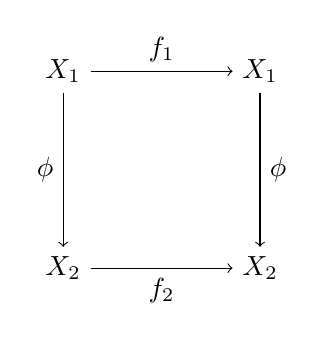
\begin{tikzpicture}[node distance=2.5cm, auto]
	\node (X) {$X_1$};
	\node (XX) [right of=X] {$X_1$};
	\node (Y) [below of=X] {$X_2$};
	\node (YY) [right of=Y] {$X_2$};
	\draw[->] (X) to node {$f_1$} (XX);
	\draw[->] (X) to node [swap] {$\phi$} (Y);
	\draw[->] (Y) to node [swap] {$f_2$} (YY);
	\draw[->] (XX) to node {$\phi$} (YY);
\end{tikzpicture}
\end{figure}
\noindent Denota-se $\phi: \Sist_1 \to \Sist_2$. Uma \emph{conjugação} (isomorfismo de sistemas dinâmicos) de $\Sist_1$ para $\Sist_2$ é uma semiconjugação $\phi: \Sist_1 \to \Sist_2$ que é invertível.
\end{definition}

\begin{figure}
\centering


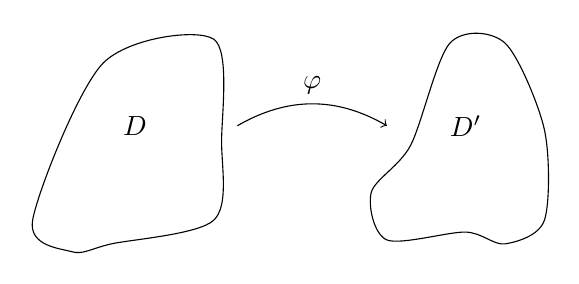
\begin{tikzpicture}
\draw plot [smooth cycle] coordinates {(5,0.25) (6,0.35) (6.5, 0.2) (7,0.5) (7,1.65) (6.5,2.75) (5.8,2.75) (5.3,1.45) (4.8,0.85) } node at (6,1.7) {$D'$};
\path[->] (3.1,1.7) edge [bend left] node[above] {$\varphi$} (5.0,1.7);
\draw plot [smooth cycle] coordinates {(1.0,.1)(1.5,.2)(2.8,.5)(2.9,1.5)(2.8,2.8)(1.4,2.5)(0.5,0.5)} node at (1.8,1.7) {$D$};
\end{tikzpicture}

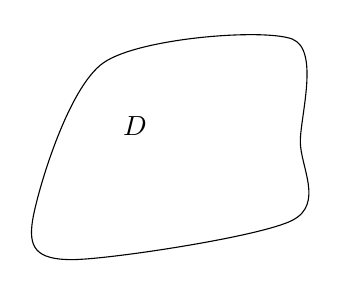
\begin{tikzpicture}
\draw plot [smooth cycle] coordinates {(1,0)(3.8,0.5)(3.9,1.5)(3.8,2.8)(1.4,2.5)(0.5,0.5)} node at (1.8,1.7) {$D$};
\end{tikzpicture}

\begin{tikzpicture}
\draw plot [smooth cycle] coordinates {(0,0)(1,1/4)(3,0)(3,3)(1,3+1/4)(0,2.5)};
\end{tikzpicture}



\end{figure}

Sempre que temos uma função sobrejetiva $\phi: X_1 \to X_2$, para todo $y \in X_2$ existe $x \in X_1$ tal que $y=\phi(x)$. Assim podemos induzir a dinâmica de $(X_1,f_1)$ em $X_2$, definindo $f_2(y) := \phi(f_1 (x))$, de modo que a dinâmica $f_2$ é uma função de $X_2$ para $X_2$ e vale $f_2 \circ \phi = \phi \circ f_1$. Isso faz com que os sistemas $(X_1,f_1)$ e $(X_2,f_2)$ sejam semiconjugados.

A partir das propriedade da conjugação, vamos deduzir alguns resultados imediatos. Podemos notar que as funções compostas ${f_1}^n$ e ${f_2}^n$ ainda satisfazem a propriedade comutativa que $f_1$ e $f_2$ satisfazem. Isso basicamente diz que em sistemas discretos, preservar a função $f$ é preservar a ação da dinâmica. Segue a proposição.

\begin{proposition}
Sejam $(X_1,f_1)$ e $(X_2,f_2)$ sistemas dinâmicos e $\phi: X_1 \to X_2$ uma semiconjugação. Então, para todo natural $n \geq 1$, vale $\phi \circ {f_1}^n = {f_2}^n \circ \phi$ (o diagrama comuta).

\begin{figure}
\centering
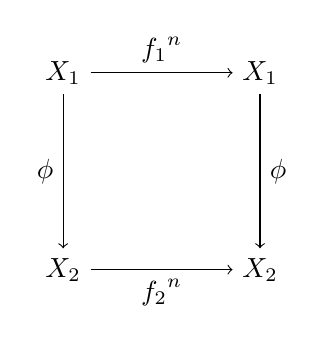
\begin{tikzpicture}[node distance=2.5cm, auto]
	\node (X) {$X_1$};
	\node (XX) [right of=X] {$X_1$};
	\node (Y) [below of=X] {$X_2$};
	\node (YY) [right of=Y] {$X_2$};
	\draw[->] (X) to node {${f_1}^n$} (XX);
	\draw[->] (X) to node [swap] {$\phi$} (Y);
	\draw[->] (Y) to node [swap] {${f_2}^n$} (YY);
	\draw[->] (XX) to node {$\phi$} (YY);
\end{tikzpicture}
\end{figure}
\end{proposition}
\begin{proof}
Vamos provar a proposição acima usando indução. Primeiro, notamos que a propriedade vale para $n = 1$ por definição. Agora, supondo que valha $\phi \circ {f_1}^{n-1} = {f_2}^{n-1} \circ \phi$, temos que
	\begin{align*}
	\phi \circ {f_1}^n & = \phi \circ ({f_1}^{n-1} \circ {f_1}) \\
						& = (\phi \circ {f_1}^{n-1}) \circ {f_1} \\
						& = ({f_2}^{n-1} \circ \phi) \circ {f_1} \\
						& = {f_2}^{n-1} \circ (\phi \circ {f_1}) \\
						& = {f_2}^{n-1} \circ ({f_2} \circ \phi) \\
						& = ({f_2}^{n-1} \circ {f_2}) \circ \phi \\
						& = {f_2}^n \circ \phi,
	\end{align*}
o que conclui a indução.
	\end{proof}

Ainda, podemos ver que a semiconjugação preserva órbitas periódicas, no sentido em que, se algum elemento do conjunto inicial tem órbita periódica, então sua imagem pela semiconjugação terá, também, órbita periódica.

\begin{proposition}[Semiconjugação preserva peridiocidade da órbita.]
Sejam $(X_1,f_1)$ e $(X_2,f_2)$ sistemas dinâmicos e $\phi: X_1 \to X_2$ uma semiconjugação. Para todo $x \in X$, se $x$ é um ponto $n$-periódico, então $\phi(x)$ é um ponto $n$-periódico. Ainda, o período mínimo de $\phi(x)$ divide o período mínimo de $x$.
\end{proposition}
\begin{proof} Seja $x \in X$ tal que $x = {f_1}^n(x)$. Pela propriedade da semiconjugação,
	\begin{align*}
	\phi(x) & = \phi({f_1}^n(x)) \\
      		  	 & = (\phi \circ {f_1}^n)(x) \\
      		  	 & = ({f_2}^n \circ \phi)(x) \\
      		  	 & = {f_2}^n(\phi(x)).
	\end{align*}
Como $\phi(x)$ é $n$-periódico, segue que seu período mínimo divide $n$.
\end{proof}


\section{Translação em grupos}

Sejam $\bm G$ um grupo e $\alpha \in G$. A translação à esquerda por $\alpha$ é a função
	\begin{align*}
	\func{E_\alpha}{G}{G}{g}{\alpha g.}
	\end{align*}

\subsection{Translação no \texorpdfstring{$\T^1$}{toro 1 dimensional}}

\begin{definition}
Seja $[\alpha] \in \T$. A \emph{rotação} por $[\alpha]$ em $\T^1$ é a função
	\begin{align*}
	\func{R_\alpha}{\T^1}{\T^1}{[x]}{[x+\alpha]}.
	\end{align*}
Uma \emph{rotação racional} é uma rotação cuja constante $\alpha$ é racional e uma \emph{rotação irracional} é uma rotação cuja constante $\alpha$ é irracional.
\end{definition}

\begin{proposition}
A dupla $(\T^1,R_\alpha)$ é um sistema dinâmico discreto revertível para todo $\alpha \in \R$ e
	\begin{enumerate}
	\item se $\alpha$ é racional, todos os pontos de $\T^1$ são periódicos;
	\item se $\alpha$ é irracional, nenhum ponto de $\T^1$ é periódico.
	\end{enumerate}
\end{proposition}
\begin{proof}
Por definição a dupla é um sistema dinâmico discreto e, como $R_{-\alpha}={R_\alpha}\inv$, segue que o sistema é invertível.
	\begin{enumerate}
	\item Seja $[x] \in \T^1$. Para mostrar que $[x]$ é periódico, devemos achar um natural $n$ tal que ${R_\alpha}^n([x]) = [x]$. A constante $\alpha$ é um número racional e, por isso, pode ser escrita em forma de fração como $\alpha = \frac{p}{q}$, sendo $p$ e $q$ inteiros e $q$ não nulo. Tomando $n = q$, e notando que $q\alpha=p$ é um inteiro, segue que
	\begin{equation*}
	{R_\alpha}^q([x]) = [x+q\alpha] = [x]
	\end{equation*}
o que mostra que $[x]$ é $q$-periódico.

	\item Seja $[x] \in \T^1$. Podemos provar a afirmação acima por contradição, notando que, se houvesse algum inteiro $n$ tal que ${R_\alpha}^n([x]) = [x]$, como ${R_\alpha}^n([x]) = [x + n\alpha]$, teríamos $n\alpha$ inteiro. Mas como $n$ é inteiro e $\alpha$ irracional, isso é impossível.
	\qedhere
	\end{enumerate}
\end{proof}

\subsection{Translação no \texorpdfstring{$\T^d$}{toro d dimensional}}

Um caso mais geral que a rotação no círculo $\T^1$ é o caso da translação no toro $\T^d$. Ela é basicamente uma rotação em cada entrada e é chamada de translação pois é a transformação induzida no espaço quociente $\T^d$ de uma translação em $\R^d$. Ela é também um caso específico de translações em grupos topológicos.

\begin{definition}
Seja $[\alpha] \in \T^d$. A \emph{translação} por $[\alpha]$ em $\T^d$ é a função
	\begin{align*}
	\func{T_\alpha}{\T^d}{\T^d}{[x]}{[x+\alpha].}
	\end{align*}
\end{definition}

%\begin{proposition}
%A dupla $(\T^d,T_\alpha)$ é um sistema dinâmico discreto revertível para todo $\alpha \in \R^d$ e
%	\begin{enumerate}
%	\item se $\alpha$ é racional, todos os pontos de $\T^1$ são periódicos;
%	\item se $\alpha$ é irracional, nenhum ponto de $\T^1$ é periódico.
%	\end{enumerate}
%\end{proposition}

\section{Expansão no \texorpdfstring{$\T^1$}{toro 1 dimensional}}

\begin{definition}
Seja $N \in \Z_{\geq 0}$. A \emph{expansão por $N$} em $\T^1$ é a função
	\begin{align*}
	\func{E_N}{\T^1}{\T^1}{[x]}{[Nx]}.
	\end{align*}
\end{definition}

Note que a função está bem definida porque $N$ é um número inteiro.


\section{Deslocamentos simbólicos}

Adotaremos a convenção de que o natural $N \in \N$ é o conjunto dos naturais menores que ele, seguindo a construção de ordinais do Von Neumann. Isso simplificará a notação. Assim temos que $N = \{0,\cdots,N-1\}$. Nesta seção consideraremos duas dinâmicas semelhantes, pois ambas agem em sequências, mas diferentes, pois uma considera sequências unilaterais e outra, bilaterais.

\subsection{Deslocamento unilateral}

Consideremos o conjunto
	\begin{equation*}
	N^{\Z_{\geq 0}} = \set{(x_i)_{i \in \Z_{\geq 0}}}{\forall i \in \Z_{\geq 0} \quad x_i \in N}
	\end{equation*}
das \emph{sequências unilaterais} em $N$ símbolos, as funções do tipo
	\begin{align*}
	\func{x}{\Z_{\geq 0}}{N}{i}{x_i}.
	\end{align*}

\begin{definition}
O \emph{deslocamento unilateral} em $N^{\Z_{\geq 0}}$ é a função
	\begin{align*}
	\func{\sigma}{N^{\Z_{\geq 0}}}{N^{\Z_{\geq 0}}}{(x_i)_{i \in \Z_{\geq 0}}}{(x_{i+1})_{i \in \Z_{\geq 0}}.}
	\end{align*}
\end{definition}

 Essa dinâmica é conhecida como \emph{deslocamento de Bernoulli} \footnote{\emph{Jacob Bernoulli} (1655 -- 1705), matemático suíço.}. Basicamente, o deslocamento desloca cada entrada de uma sequência $(x_0,x_1,x_2,\ldots)$ à esquerda, levando-a para sequência $(x_1,x_2,x_3,\ldots)$. Claramente essa função não é invertível, logo o sistema dinâmico formado por ela não é invertível. Ressaltamos isso na proposição a seguir.

\begin{proposition}
A dupla $(N^{\Z_{\geq 0}},\sigma)$ é um sistema dinâmico discreto irrevertível.
\end{proposition}

\begin{proposition}
Seja $k \in \Z_{\geq 0}$. Uma sequência unilateral $(x_i)_{i \in \Z_{\geq 0}} \in N^{\Z_{\geq 0}}$ é um ponto $k$-periódico de $(N^{\Z_{\geq 0}},\sigma)$  se, e somente se, para todo $i \in \Z_{\geq 0}$, vale $x_i = x_{i+k}$.
\end{proposition}
\begin{proof}
Se vale $x_i = x_{i+k}$ para todo $i \in \Z_{\geq 0}$, a sequência $(x_i)_{i \in \Z_{\geq 0}}$ claramente será $k$-periódica, pois
	\begin{equation*}
	\sigma^k((x_i)_{i \in \Z_{\geq 0}}) = (x_{i+k})_{i \in \Z_{\geq 0}} = (x_i)_{i \in \Z_{\geq 0}}.
	\end{equation*}

Por outro lado, se $(x_i)_{i \in \Z_{\geq 0}}$ tiver órbita periódica, valerá
	\begin{equation*}
	\sigma^k((x_i)_{i \in \Z_{\geq 0}}) = (x_i)_{i \in \Z_{\geq 0}}
	\end{equation*}
para algum $k$. Nesse caso, teremos que $x_i = x_{i+k}$ para todo $i \in \Z_{\geq 0}$.
\end{proof}

\begin{proposition}
A função
	\begin{align*}
	\func{\phi}{N^{\Z_{\geq 0}}}{\T^1}{(x_i)_{i \in \Z_{\geq 0}}}{\left[\sum_{i \in \Z_{\geq 0}} \frac{x_i}{N^{i+1}}\right]}
	\end{align*}
é uma semiconjugação de $(N^{\Z_{\geq 0}},\sigma)$ para $(\T^1,E_N)$.
\end{proposition}
\begin{proof}
Seja $(x_i)_{i \in \Z_{\geq 0}} \in N^{\Z_{\geq 0}}$. Então
	\begin{align*}
	\phi \circ \sigma((x_i)_{i \in \Z_{\geq 0}}) &= \phi((x_{i+1})_{i \in \Z_{\geq 0}}) \\
			&=\left[\sum_{i \in \Z_{\geq 0}} \frac{x_{i+1}}{N^{i+1}}\right] \\
			&=\left[N\sum_{i \in \Z_{\geq 0}} \frac{x_{i+1}}{N^{i+2}}\right] \\
			&=\left[N \left(\frac{x_0}{N} + \sum_{i \in \Z_{>0}} \frac{x_{i}}{N^{i+1}}\right)\right] \\
			&=\left[N \sum_{i \in \Z_{\geq 0}} \frac{x_{i}}{N^{i+1}}\right] \\
			&=E_N \circ \phi((x_i)_{i \in \Z_{\geq 0}}).
	\end{align*}
Somamos $x_0$ na quarta linha pois é um inteiro, não altera a classe de equivalência.
\end{proof}

Notemos que a função $\phi$ não é uma conjugação porque não é invertível --- existe mais de uma representação $N$-ária para alguns números reais em $[0,1]$, portanto mais de uma sequência em $N^{\Z_{\geq 0}}$ que o representa. No entanto, veremos mais à frente que isso não será problema quando considerarmos sistemas dinâmicos de medida, pois o conjunto desses pontos problemáticos terá medida nula e, portanto, a conjugação poderá ser definida. Isso será importante pois significa que os dois sistemas são o mesmo sob a ótica de sistemas dinâmicos de medida.


\subsection{Deslocamento bilateral}

Consideremos o conjunto
	\begin{equation*}
	N^\Z = \set{(x_i)_{i \in \Z}}{\forall i \in \Z \quad x_i \in N}
	\end{equation*}
das \emph{sequências bilaterais} em $N$ símbolos, as funções do tipo
	\begin{align*}
	\func{x}{\Z}{N}{i}{x_i}.
	\end{align*}

\begin{definition}
O \emph{deslocamento bilateral (à esquerda)} em $N^\Z$ é a função
	\begin{align*}
	\func{\sigma}{N^\Z}{N^\Z}{(x_i)_{i \in \Z}}{(x_{i+1})_{i \in \Z}.}
	\end{align*}
O \emph{deslocamento bilateral à direita} é $\sigma\inv$.
\end{definition}


\begin{proposition}
A dupla $(N^\Z,\sigma)$ é um sistema dinâmico discreto revertível.
\end{proposition}

\subsection{Subdeslocamentos}

Os deslocamentos definidos anteriormente são deslocamentos completos, no sentido de que todas as sequências são consideradas no sistema. É possível, porém, selecionar subconjuntos dessas sequências tal que o deslocamento ainda está bem definido nelas. Definimos que cada entrada de uma sequência $(x_i)_{i \in \Z} \in N^\Z$ tem entradas em $\{0,\ldots,N-1\}$. Esses subconjuntos são escolhidos a partir de uma regra que indica qual entrada de uma sequência pode ser seguida de qual outra entra --- por exemplo, para $N=9$, sequências em que uma entrada $4$ só pode ser seguida de uma entrada $2$ ou uma entrada $8$. Para ter toda a informação necessária, essas sequências são definidas a partir de uma \emph{matriz de adjacência}, uma matriz que indica qual entrada pode ser adjacente a qual outra.

\begin{definition}
Uma \emph{matriz de adjacência} de ordem $N$ é uma matriz $A \in \M_N(\Z)$ de entradas $0$ ou $1$ tal que $a_{i,j}=0$ se uma entrada com valor $i$ não pode ser seguida de uma entrada com valor $j$ e $a_{i,j}=1$ se uma entrada de valor $i$ pode ser seguida de uma entrada de valor $j$.
\end{definition}

\begin{definition}
Sejam $N \in \Z_{>0}$ e $A$ uma matriz de adjacência de ordem $N$. O conjunto das sequências de $N^\Z$ \emph{admissíveis} por $A$ é o conjunto
	\begin{equation*}
	N^\Z|_A := \set{(x_i)_{i \in \Z}}{\forall i \in \Z, a_{x_i,x_{i+1}}=1}.
	\end{equation*}
O conjunto das sequências de $N^{\Z_{\geq 0}}$ restritas por $A$ é o conjunto
	\begin{equation*}
	N^{\Z_{\geq 0}}|_A := \set{(x_i)_{i \in {\Z_{\geq 0}}}}{\forall i \in {\Z_{\geq 0}}, a_{x_i,x_{i+1}}=1}.
	\end{equation*}
O \emph{subdeslocamento bilateral} com \emph{matriz de adjacência} $A$ é a função $\sigma|_A := \sigma|_{N^\Z|_A}$ e o \emph{subdeslocamento unilateral} com \emph{matriz de adjacência} $A$ é a função $\sigma|_A := \sigma|_{N^{\Z_{\geq 0}}|_A}$. Os sistemas $(N^\Z|_A,\sigma|_A)$ e $(N^{\Z_{\geq 0}}|_A,\sigma|_A)$ são \emph{sistemas de deslocamento parcial} e a matriz $A$ é a \emph{matriz de adjacência} dos sistemas.
\end{definition}

Esses sistemas também são conhecidos como \emph{cadeias de Markov} \footnote{\emph{Andrei Andreyevich Markov} (1856 -- 1922), matemático russo.}.

\begin{proposition}
Sejam $N \in \Z_{>0}$ e $A$ uma matriz de adjacência de ordem $N$. A inclusão $\iota\colon N^\Z|_A \to N^\Z$ é uma semiconjugação do sistema $(N^\Z|_A,\sigma|_A)$ para o sistema $(N^\Z|_A,\sigma|_A)$.
\end{proposition}
\begin{proof}
Queremos mostrar que $\iota \circ \sigma|_A = \sigma \circ \iota$. Seja $(x_i)_{i \in \Z} \in N^\Z|_A$. Então
	\begin{align*}
	\iota \circ \sigma|_A ((x_i)_{i \in \Z}) &= \iota (\sigma|_A((x_i)_{i \in \Z})) \\
		&= \iota((x_{i+1})_{i \in \Z}) \\
		&= (x_{i+1})_{i \in \Z} \\
		&= \sigma ((x_i)_{i \in \Z}) \\
		&= \sigma (\iota((x_i)_{i \in \Z})) \\
		& =\sigma \circ \iota ((x_i)_{i \in \Z}).
	\end{align*}
\end{proof}

O mesmo vale para os sistemas unilaterais. A partir da matriz da matriz de adjacência podemos determinar quantos pontos periódicos de um determinado período existem.

\begin{proposition}
Sejam $p \in \Z_{>0}$ e $(N^\Z|_A,\sigma|_A)$ um sistema de subdeslocamento com matriz de adjacência $A$. A quantidade de pontos $p$-periódicos de $(N^\Z|_A,\sigma|_A)$ é $\tr(A^p)$.
\end{proposition}
\begin{proof}
Sabemos que $(x_i)_{i \in \Z}$ é $p$-periódico se, e somente se, para todo $i \in \Z$ vale $x_i = x_{i+p}$. Sendo assim, procuramos os pontos da forma
	\begin{equation*}
	(\ldots,x_{i_0},x_{i_1},\ldots,x_{i_{p-2}},x_{p-1},\ldots)
	\end{equation*}
e portanto devemos achar os vetores $(i_0,\ldots,i_{p-1}) \in N^p$ tais que a sequência de entradas
	\begin{equation*}
	i_0 \rightarrow i_1 \rightarrow \cdots i_{p-2} \cdots i_{p-1}
	\end{equation*}
é uma sequência permitida pela matriz de adjacência. Isso é equivalente a termos
	\begin{equation*}
	\bigtimes_{k=0}^{p-2} a_{i_k,i_{k+1}} = a_{i_0,i_1}a_{i_1,i_2}\cdots a_{i_{p-3},i_{p-2}}a_{i_{p-2},i_{p-1}} = 1,
	\end{equation*}
pois esse produto é $1$ se, e somente se todos os fatores são $1$. Assim, a quantidade de pontos periódicos é a soma de todos esses produtos
	\begin{align*}
	\abs{\Per[p](\sigma_A)} &= \sum_{(i_0,\ldots,i_{p-1}) \in N^p} \bigtimes_{k=0}^{p-2} a_{i_k,i_{k+1}} \\
		&= \sum_{i_0=0}^{N-1} \sum_{(i_1,\ldots,i_{p-1}) \in N^{p-1}} \bigtimes_{k=0}^{p-2} a_{i_k,i_{k+1}} \\
		&= \sum_{i_0=0}^{N-1} (A^p)_{i_0,i_0} = \tr(A^p).
	\end{align*}
\end{proof}

\subsection{Itinerários}

\begin{definition}
Sejam $(X,f)$ um sistema dinâmico discreto, $\mathcal P=(P_i)_{i \in N}$ uma partição finita de $X$ ($N \in \N$) e $x \in X$. O \emph{itinerário} de $x$ com respeito a $\mathcal P$ é a sequência
%	\begin{equation*}
%	(\mathcal P\inv(f^i(x)))_{i \in T};
%	\end{equation*}
%ou seja, é a sequência
$(x_t)_{t \in T} \in N^T$ tal que $x_t=k$ se, e somente se, $f^t(x) \in P_k$.
\end{definition}

\begin{proposition}
Sejam $(X,f)$ um sistema dinâmico discreto, $\mathcal P=(P_i)_{i \in N}$ uma partição finita de $X$ e $\phi: X \to N^T$ a função que leva $x \in X$ em seu itinerário com respeito a $\mathcal P$. Então
	\begin{equation*}
	\phi \circ f = \sigma \circ \phi.
	\end{equation*}
\end{proposition}
\begin{proof}
Sejam $x \in X$ e $\phi(x) = (x_t)_{t \in T}$. Então $\phi(f(x)) = (x_{t+1})_{t \in T}$, pois $f^t(f(x)) = f^{t+1}(x)$. Portanto
	\begin{equation*}
	\phi \circ f(x) = \phi(f(x)) = (x_{t+1})_{t \in T} = \sigma ((x_t)_{t \in T}) = \sigma(\phi(x)) = \sigma \circ \phi (x),
	\end{equation*}
o mostra que $\phi \circ f = \sigma \circ \phi$.
\end{proof}

A imagem $\phi(X)$ é invariante por $\sigma$, pois
	\begin{equation*}
	\sigma(\phi(X)) = \phi(f(X)) = \phi(X),
	\end{equation*}
de modo que $\phi$ é uma semiconjugação de $X$\(X\) para $\phi(X)$, pois satisfaz a propriedade comutativa e é sobrejetiva por definição. Nem sempre tem-se $\phi$ injetiva, isso depende da partição e do sistema que se estuda. Ainda, nem sempre $\phi$ preserva as estruturas adicionais de $X$. Nas seções posteriores serão apresentadas partições que preservam tais estruturas.

Sejam $(X,f)$ um sistema dinâmico discreto, $\mathcal P=(P_i)_{i \in N}$ uma partição finita de $X$ e $(x_t)_{t \in T} \in N^T$. O conjunto
	\begin{equation*}
	\bigcap_{t \in T} f^{-t}(P_{x_t}).
	\end{equation*}
é o conjunto dos pontos $x \in X$ tal que $f^t(x) \in P_{x_t}$ para todo $t \in T$, pois $f^t(x) \in P_{x_t}$ se, e somente se, $x \in f^{-t}(P_{x_t})$; ou seja, o conjunto de todos os pontos tais que $\phi(x)=(x_t)_{t \in T}$.

%	\begin{equation*}
%	f^{-t}(P_k) = C_{t}[k] \cap \phi(X)
%	\end{equation*}

%%%%%%%%%%%%%%%%%%%%%%%%%%%%%%%%%%%%%%%%%%%%%
%%%%%%%%%%%%%%%%%%%COMENTÁRIO%%%%%%%%%%%%%%%%%%%
%%%%%%%%%%%%%%%%%%%%%%%%%%%%%%%%%%%%%%%%%%%%%
\begin{comment}

\subsection{Ferradura}

Nesta seção, trataremos de um sistema dinâmico conhecido por Ferradura de Smale. O conjunto usado nesta seção será criado a partir de um conjunto $D \subseteq \R^2$. Esse conjunto $D$ é particionado em cinco conjuntos: $D = D_1 \cup D_2 \cup D_3 \cup D_4 \cup D_5$. Os conjuntos $D_2, D_3, D_4$ formam um quadrado unitário $R := D_2 \cup D_3 \cup D_4$ e os conjuntos $D_1,D_5$ são semicírculos de diâmetro unitário, como na figura abaixo.

\begin{figure}[!ht]
  \centering
	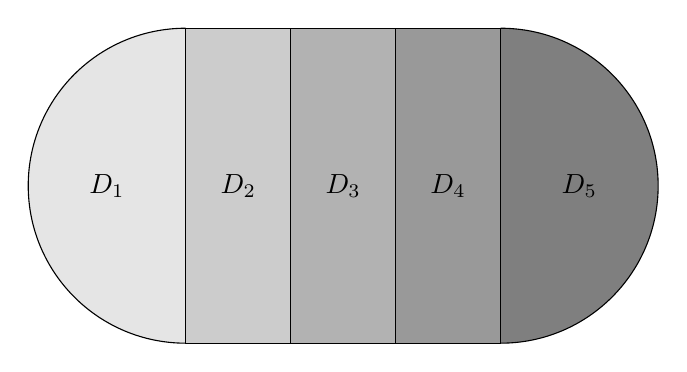
\begin{tikzpicture}[scale=2]

		\filldraw[fill=black, fill opacity=0.1] (-1,1) arc [start angle=90, end angle=270, radius=1];
		\filldraw[fill=black, fill opacity=0.2]	(-1,-1) rectangle (-0.333,1);
		\filldraw[fill=black, fill opacity=0.3]	(-0.333,-1) rectangle (0.333,1);
		\filldraw[fill=black, fill opacity=0.4]	(0.333,-1) rectangle (1,1);
		\filldraw[fill=black, fill opacity=0.5]	(1,-1) arc [start angle=-90, end angle=90, radius=1];

		\foreach \x/\xtext in {-1.5/D_1,-0.666/D_2,0/D_3,0.666/D_4,1.5/D_5}
		\draw (\x cm,0pt) -- (\x cm,0pt) node {$\xtext$};

		\end{tikzpicture}
  \caption{O conjunto $D = D_1 \cup R \cup D_5$}
\end{figure}

Associamos ao conjunto $D$ o endomorfismo diferenciável $f: D \to D$ que estica e entorta o conjunto $D$ nele mesmo, como na figura a seguir.

\begin{figure}[!ht]
  \centering
	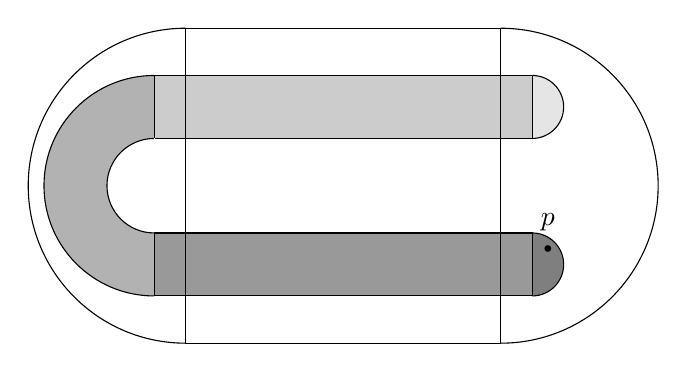
\begin{tikzpicture}[scale=2]
		\draw (-1,-1) rectangle (1,1);
		\draw (-1,1) arc [start angle=90, end angle=270, radius=1];
		\draw (1,-1) arc [start angle=-90, end angle=90, radius=1];

		\filldraw[fill=black, fill opacity=0.1] (1.2,0.3) arc [start angle=-90, end angle=90, radius=0.2];
		\filldraw[fill=black, fill opacity=0.2] (1.2,0.3) rectangle (-1.2,0.7);
		\filldraw[fill=black, fill opacity=0.3] (-1.2,0.7) arc [start angle=90, end angle=270, radius=0.7] ;
		\filldraw[fill=white, fill opacity=1] (-1.2,0.3) arc [start angle=90, end angle=270, radius=0.3];
		\draw[draw=white] (-1.2,0.3) -- (-1.2,-0.3);
		\filldraw[fill=black, fill opacity=0.4] (1.2,-0.3) rectangle (-1.2,-0.7);
		\filldraw[fill=black, fill opacity=0.5] (1.2,-0.7) arc [start angle=-90, end angle=90, radius=0.2];

		\draw (1.3,-0.4) node {{\tiny $\bullet$}};
		\draw (1.3,-0.35) node[anchor=south] {{$p$}};

		\end{tikzpicture}
  \caption{A imagem de $D$ sob o endomorfismo $f$}
\end{figure}

Assuma que $f$ estica $D_2 \cup D_4$ uniformemente na direção horizontal por um fator $\med > 2$ e contrai uniformemente $D_2 \cup D_4$ na direção vertical por um fator $\lambda < \frac{1}{2}$. Ainda, note que, pelo teorema do ponto fixo de Brouwer, existe um ponto fixo $p \in f(D_5)$, pois $f(D_5) \in D_5$.

Queremos estudar esse sistema usando uma conjugação com o deslocamento simbólico. Vamos definir os seguintes conjuntos:
	\begin{equation*}
	R_0 := f(D_2) \cap R \qquad \qquad R_1 := f(D_4) \cap R.
	\end{equation*}

Note que $f(R) \cap R = R_0 \cup R_1$. A partir desses conjuntos, vamos definir uma sequência de conjuntos da mesma forma. Assim como $f(R) \cap R$ consiste em dois retângulos, que nomeamos $R_0$ e $R_1$, o conjunto $f^2(R) \cap f(R) \cap R = f^2(R) \cap R$ consiste em quatro retângulos que nomearemos $R_{00}, R_{01}, R_{10}$ e $R_{11}$. Vale notar que a altura dos retângulos $R_0$ e $R_1$ é $\lambda$ e a dos retângulos $R_{00}, R_{01}, R_{10}$ e $R_{11}$ é $\lambda^2$.

\begin{figure}[!ht]
\centering
	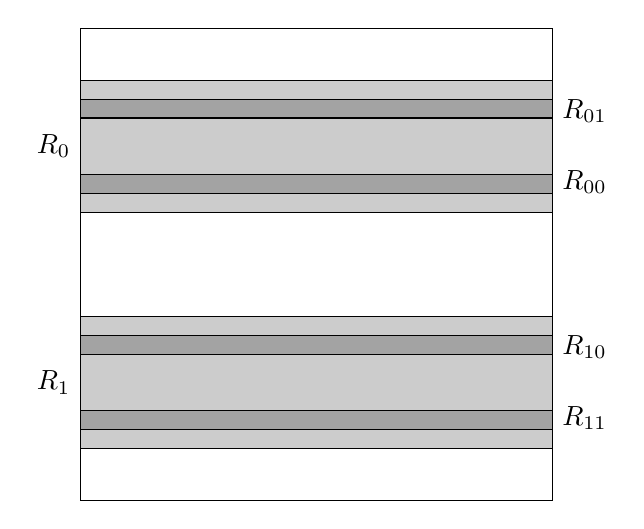
\begin{tikzpicture}[scale=3]

	\draw (-1,-1) rectangle (1,1);
	\filldraw[fill=black, fill opacity=0.2] (-1,0.3) rectangle (1,0.7);
	\filldraw[fill=black, fill opacity=0.2] (-1,-0.3) rectangle (1,-0.7);

	\filldraw[fill=black, fill opacity=0.2] (-1,0.62) rectangle (1,0.78);
	\filldraw[fill=black, fill opacity=0.2] (-1,0.38) rectangle (1,0.22);
	\filldraw[fill=black, fill opacity=0.2] (-1,-0.62) rectangle (1,-0.78);
	\filldraw[fill=black, fill opacity=0.2] (-1,-0.38) rectangle (1,-0.22);


	\draw (-1,0.5) node[anchor=east] {{$R_0$}};
	\draw (-1,-0.5) node[anchor=east] {{$R_1$}};

	\draw (1,0.65) node[anchor=west] {{$R_{01}$}};
	\draw (1,0.35) node[anchor=west] {{$R_{00}$}};
	\draw (1,-0.35) node[anchor=west] {{$R_{10}$}};
	\draw (1,-0.65) node[anchor=west] {{$R_{11}$}};

	\end{tikzpicture}
	\caption{O quadrado $R$ e conjuntos $R_\omega$ horizontais usados na conjugação}
\end{figure}

De modo geral, para qualquer sequência finita $\omega = (\omega_0,\omega_1, \ldots, \omega_n) \in 2^{n+1}$ de zeros e uns, definimos
	\begin{equation*}
	R_\omega := \bigcap_{i=0}^n f^i(R_{\omega_i}) = R_{\omega_0} \cap f(R_{\omega_1})  \cap f^2(R_{\omega_2}) \cap \cdots \cap f^n(R_{\omega_n}),
	\end{equation*}
que será um retângulo horizontal de altura $\lambda^n$ e $f^n(R) \cap R$ será a união dos $2^n$ possíveis retângulos dessa forma. Para uma sequência unilateral $\omega = (\omega_i)_{i \in \Z_{\geq 0}} \in 2^{\Z_{\geq 0}}$, o retângulo $R_\omega$ é definido como
	\begin{equation*}
	R_\omega := \bigcap_{i \in \Z_{\geq 0}} f^i(R_{\omega_i}).
	\end{equation*}

Construiremos, de modo semelhante, retângulos verticais a parir da função inversa $f^{-1}$. Note que $f^{-1} (R_0) = f^{-1} (R) \cap D_2$ e $f^{-1} (R_1) = f^{-1} (R) \cap D_4$ são retângulos verticais de largura $\med^{-1}$. Assim, para uma sequência finita $\omega = (\omega_1, \ldots, \omega_n) \in 2^n$ de zeros e uns, definimos
	\begin{equation*}
	R'_\omega := \bigcap_{i=1}^n f^{-i}(R_{\omega_i}) = f^{-1}(R_{\omega_1}) \cap f^{-2}(R_{\omega_2}) \cap \cdots \cap f^{-n}(R_{\omega_n}),
	\end{equation*}
que será um retângulo vertical de largura $\med^{-n}$ e $f^{-n}(R) \cap R$ será a união dos $2^n$ possíveis retângulos dessa forma. Para uma sequência unilateral $\omega = (\omega)_{i \in \Z_{>0}} \in 2^{\Z_{>0}}$, definimos
	\begin{equation*}
	R'_\omega := \bigcap_{i \in \Z_{>0}} f^{-i}(R_{\omega_i}).
	\end{equation*}

\begin{definition}
A \textit{ferradura} é o conjunto $F$ definido como
	\begin{equation*}
	F := \bigcap_{i \in \Z} f^i(R).
	\end{equation*}
\end{definition}

Lembrando das definições dos retângulos no começo da seção, podemos perceber que $F$ é a união de todos os conjuntos $R_\omega \cap R'_\omega$, com $\omega$ variando em $2^\Z$.

\begin{definition}
A conjugação $\phi$ do sistema da ferradura $(H,f)$ para o deslocamento bilateral $(2^\Z,\sigma\inv)$ é definida como
	\begin{align*}
	\func{\phi}{F}{2^\Z}{x}{(x_i)_{i \in \Z}}
	\end{align*}
tal que $x_i = k$ se $f^i(x) \in R_k$.
\end{definition}

\begin{proposition}
A função $\phi$ é uma conjugação do sistema $(F,f)$ para o sistema $(2^\Z,\sigma\inv)$.
\end{proposition}
\begin{proof}
Primeiramente, vamos demonstrar que a função $\phi$ é bijetiva. Para mostrar a sobrejetividade, consideremos $(x_i)_{i \in \Z} \in 2^\Z$. Definamos as sequências positiva e negativa de $(x_i)$ como as sequências unilaterais
	\begin{equation*}
	(x_i)^+ := (x_0,x_1,\ldots) \e (x_i)^- := (x_{-1},x_{-2},...).
	\end{equation*}

Consideremos os retângulos horizontais $R_{x_0},  R_{(x_0,x_1)}, R_{(x_0,x_1,x_2)}, \ldots \ $. Esses retângulos estão cada um contido no anterior, $R_{x_0} \supset  R_{(x_0,x_1)} \supset R_{(x_0,x_1,x_2)} \supset \ldots \ $. Se consideramos suas interseções com alguma reta vertical em $R$, temos intervalos encaixados $I_{x_0}, I_{(x_0,x_1)}, I_{(x_0, x_1, x_2)}, \ldots$, respectivamente, que são intervalos fechados e satisfazem $I_{x_0} \supset I_{(x_0,x_1)} \supset I_{(x_0, x_1, x_2)} \supset \ldots \ $. Portanto, pelo teorema dos intervalos encaixados, concluímos que a interseção desses intervalos é não vazia: $I_{x_0} \cap I_{(x_0,x_1)} \cap I_{(x_0, x_1, x_2)} \cap \ldots \neq \emptyset$. Ainda, podemos concluir que existe um único elemento pertencente a essa interseção, pois o comprimento de cada intervalo é a altura de seu respectivo retângulo e, portanto, diminui geometricamente por um fator de $\lambda < 1$, tal que o comprimento final da interseção é 0. Como esse argumento vale para qualquer reta vertical em $R$, concluímos que $R_{(x_n)^+} = \bigcap_{i \in \N} f^i(R_{x_i})$, que é o conjunto de todos esses pontos, é uma reta horizontal em $R$. Da mesma forma, consideramos os retângulos verticais $R'_{x_{-1}},  R'_{(x_{-1},x_{-2})}, R'_{(x_{-1},x_{-2},x_{-3})}, \ldots \ $. Suas interseções com uma reta horizontal em $R$ são intervalos encaixados $I'_{x_{-1}}, I'_{(x_{-1},x_{-2})}, I'_{(x_{-1}, x_{-2}, x_{-3})}, \ldots$, respectivamente, que são intervalos fechados e e satisfazem $I'_{x_{-1}} \supset I'_{(x_{-1},x_{-2})}  \supset I'_{(x_{-1}, x_{-2}, x_{-3})} \supset \ldots \ $. Pelo teorema dos intervalos encaixados, concluímos que a interseção desses intervalos é não vazia e, como anteriormente, como o comprimento de cada intervalo é a largura de seu respectivo retângulo e, portanto, diminui geometricamente por um fator de $\med^{-1} < 1$, a interseção desses intervalos terá um único elemento. Novamente, esse argumento vale para qualquer reta horizontal em $R$, e concluímos que $R'_{(x_n)^-} = \bigcap_{i \in \N \setminus \{0\}} f^{-i}(R_{x_{-i}})$, o conjunto de todos esses pontos, é uma reta vertical em $R$. Por fim, notamos que as retas horizontal e vertical definidas acima se tocam em um único ponto $x$. Isso que dizer que $R_{(x_n)^+} \cap R'_{(x_n)^-} = \{x\}$. Portanto, por construção, vale que $f^n(x) \in R_{x_n}$ para todo inteiro $n$ e, assim, concluímos que $\phi(x) = (x_i)_{i \in \Z}$. Isso prova a sobrejetividade.

Para mostrar a injetividade, consideremos dois elementos $a,b \in F$ e sejam suas imagens $\phi(a) = (a_n)_{n \in \Z}$ e $\phi(b) = (b_n)_{n \in \Z}$. Suponhamos que $(a_n)_{n \in \Z} = (b_n)_{n \in \Z}$. Nesse caso, sabemos que $R_{(a_n)_{n \in \Z}} = R_{(b_n)_{n \in \Z}}$ e que, portanto, $a$ e $b$ pertencem a $R_{(a_n)_{n \in \Z}}$. Mas foi demonstrado acima que, dado $\omega \in 2^\Z$, o conjunto $R_\omega$ tem somente um elemento, o que implica que $a=b$.

Vamos agora mostrar que vale a relação comutativa $\phi \circ f = \sigma \circ \phi$. Seja $x \in F$ e $\phi(x) = (x_n)_{n \in \Z}$. Nesse caso, sabemos que $x \in R_{(x_n)_{n \in \Z}}$. Aplicando $f$ a $R_{(x_n)}$, temos
	\begin{align*}
	f(R_{(x_n)_{n \in \Z}}) &= f\left( \bigcap_{i \in \Z}f^i(R_{x_i})\right) \\
				&= \bigcap_{i \in \Z}f^{i+1}(R_{x_i}) \\
				&= \bigcap_{i \in \Z}f^i(R_{x_{i-1}}) \\
				&= R_{(x_{n-1})_{n \in \Z}}.
	\end{align*}
Mas isso implica que $f(x) \in R_{(x_{n-1})_{n \in \Z}}$ e, portanto, pela bijetividade de $\phi$, temos $\phi(f(x)) = (x_{n-1})_{n \in \Z}$. Por outro lado, como $\phi(x) = (x_n)_{n \in \Z}$, temos $\sigma(\phi(x)) = (x_{n-1})_{n \in \Z}$. Logo $\phi \circ f = \sigma \circ \phi$.
\end{proof}

\end{comment}
%%%%%%%%%%%%%%%%%%%%%%%%%%%%%%%%%%%%%%%%%%%%%
%%%%%%%%%%%%%%%%%%%COMENTÁRIO%%%%%%%%%%%%%%%%%%%
%%%%%%%%%%%%%%%%%%%%%%%%%%%%%%%%%%%%%%%%%%%%%

\subsection{Automorfismos hiperbólicos no \texorpdfstring{$\T^2$}{toro 2-dimensional}}

Após o estudo de duas dinâmicas envolvendo o círculo, a dinâmica de rotação na  e a de expansão, voltamos nossa atenção nesta seção a um novo objeto geométrico: o toro. O sistema dinâmico a ser estudado nesta seção tem como conjunto o toro $\T^2$, descrito acima, e a dinâmica que age nele é chamada de automorfismo hiperbólico. Essa função é dada por uma matriz de dimensão $2 \times 2$ com algumas características específicas. Como a próxima definição dependente muito da utilização de matrizes, convém definir algumas coisas sobre elas antes de abordarmos a dinâmica no toro. Denotaremos uma matriz sempre com uma letra maiúscula e seus elementos com a respectiva letra minúscula acompanhados dos índices; escrevemos $A = [a_{i,j}]$. A dimensão de uma matriz será explicitada somente quando necessário e será simplificada para matrizes quadradas, como em $A_{2x2}=A_{2}$. Denotaremos o determinante de uma matriz $A$ por $|A|$ ou $\det(A)$ e sua matriz inversa por $A^{-1}$. Convenções esclarecidas, definimos o automorfismo.

\begin{definition}
Seja $A \in \SL_2(\Z)$ uma matriz cujos autovalores têm valor absoluto não unitário. O \textit{automorfismo hiperbólico} no toro é definido a partir de $A$ como
	\begin{align*}
	\func{[A]}{\T^2}{\T^2}{[x]}{[Ax]}.
	\end{align*}
\end{definition}

Para justificar a nomenclatura dessa classe de funções como automorfismos hiperbólicos, devemos demonstrar algumas propriedades tanto da matriz $A$ como da função $[A]$. A matriz é dada por
	\begin{equation*}
	A = \begin{bmatrix}
		a_{11} & a_{12} \\
		a_{21} & a_{22}
		\end{bmatrix}
	\end{equation*}
As entradas devem ser inteiras para que a operação $[A](x)$ esteja bem definida no toro. Isso ocorre pois, para todo $y \in [x]$, temos $y = x + k$, com $k \in \Z^2$, e segue que
	\begin{equation*}
	[Ay] = [A(x+k)] = [Ax + Ak] = [Ak],
	\end{equation*}
pois $Ak \in \Z^2$.

Devemos justificar por que essa função é um automorfismo. Claramente, a função $[A]$ é um endomorfismo por ter como domínio e contradomínio o mesmo conjunto. Para ser um automorfismo, deve ser também um isomorfismo. Isso ocorre porque o determinante da matriz $A$ é igual a 1, o que faz com que sua matriz inversa
	\begin{equation*}
	A^{-1} = \begin{bmatrix}
		a_{22} & -a_{12} \\
		-a_{21} & a_{11}
		\end{bmatrix}
	\end{equation*}
seja também uma matriz com entradas inteiras, determinante unitário e autovalores distintos, e a função inversa $L_{A^{-1}} := [A^{-1}x]$ esteja bem definida no toro. O automorfismo $[A]$ recebe o nome de hiperbólico porque matrizes cujos autovalores têm valor absoluto diferente de 1 recebem esse nome. Vale notar, por fim, que para todo inteiro $k$, vale
	\begin{equation*}
	[A]^k = [A^k].
	\end{equation*}

A partir da definição da matriz $A$, podemos deduzir algumas características imediatas dos autovalores, autovetores e determinante da matriz.

\begin{proposition}
Seja $A \in \SL_2(\Z)$ uma matriz cujos autovalores têm valor absoluto não unitário. Então
	\begin{enumerate}
	\item Os autovalores de $A$ são
		\begin{align*}
		\lambda_+ &:= \frac{1}{2}\left(a_{11}+a_{22} + \sqrt{(a_{11}+a_{22})^2 - 4}\right) \\
		\lambda_- &:= \frac{1}{2}\left(a_{11}+a_{22} - \sqrt{(a_{11}+a_{22})^2 - 4}\right)
		\end{align*}
e as entradas de $A$ satisfazem $a_{11}+a_{22} \neq \pm 2$, $a_{12} \neq 0$ e $a_{21} \neq 0$.
	\item Os autovalores de $\lambda_+$ e $\lambda_-$ são irracionais;
	\item Os autovetores de $A$ são
	\begin{align*}
	v_{\lambda_+} &:= \left(1, \frac{\lambda_+ -a_{11}}{a_{12}}\right) \\
	 v_{\lambda_-} &:= \left(1, \frac{\lambda_- -a_{11}}{a_{12}}\right) .
	\end{align*}
	\end{enumerate}


	\end{proposition}
\begin{proof}
	\begin{enumerate}
	\item Primeiro, notemos que o polinômio característico de $A$ será
	\begin{equation*}
	\chi_A(\lambda) = \lambda^2 -(a_{11}+a_{22})\lambda+1.
	\end{equation*}
Assim, isolando $\lambda$ pela fórmula quadrática, obtemos $\lambda_+$ e $\lambda_-$ como no enunciado. Para termos $\lambda_+ \neq \lambda_-$, devemos ter $\sqrt{(a_{11}+a_{22})^2 - 4} \neq 0$, o que implica $a_{11}+a_{22} \neq \pm 2$. Por fim, se $a_{12} = 0$ ou $a_{21} = 0$, temos $a_{12}a_{21} = 0$, o que implica $\det A = a_{11}a_{22} = 1$. Teríamos, portanto, $a_{22} = \frac{1}{a_{11}}$, mas como todas entradas são inteiras, isso implicaria $a_{11} = a_{22} = \pm 1$, e teríamos a contradição $a_{11} + a_{22} = \pm 2$.

	\item Vamos demonstrar o lema por absurdo. Primeiramente notamos que os autovalores de $A$ devem ser reais pois, caso contrário, seriam complexos conjugados. Então seu produto seria $\lambda_+ \lambda_- = |\lambda_+|^2 = |\lambda_-|^2 = \pm 1$. Mas isso é absurdo, pois os módulos dos autovalores são diferentes de $1$. Consideremos o autovalor $\lambda_{+}$ e suponhamos que ele é um número racional. Ao isolar a raiz na expressão de $\lambda_{+}$ obtemos
	\begin{equation*}
	\sqrt{(a_{11}+a_{22})^2 - 4} = 2\lambda_{+}-(a_{11}+a_{22}).
	\end{equation*}
Mas $(a_{11}+a_{22})^2 - 4$ é inteiro e sabemos que a raiz de um número inteiro é inteira ou irracional. Devemos ter $2\lambda_{+}-(a_{11}+a_{22})$ inteiro, portanto. Fazendo $x = a_{11}+a_{22}$ e $y = 2\lambda_{+}-(a_{11}+a_{22})$, devemos ter $x$ e $y$ inteiros e, rearrumando a equação,
	\begin{equation*}
	x^2 - y^2 = 4.
	\end{equation*}
De fato, para achar uma solução inteira da equação acima, notamos que $x^2 - y^2 = (x+y)(x-y)$ e temos três opções, já que $4=2 \cdot 2 = 4 \cdot 1$. A primeira é $x+y = 2$ e $x-y = 2$. Isso implica $x+y = x-y$, que implica $y=0$ e, por fim, $a_{11}+a_{22} = x = 2$, o que contradiz o item anterior da proposição. As outras duas opções são $x+y = 4$ e $x-y = 1$ ou $x+y = 1$ e $x-y = 4$. Ambas, no entanto, implicam $x = \frac{5}{2}$, o que é um absurdo porque $x = a_{11}+a_{22}$ é um número inteiro. Assim, concluímos que o autovalor $\lambda_{+}$ é irracional. Como $\lambda_- = \frac{1}{\lambda_+}$, ambos autovalores são ambos irracionais.

	\item Para calcular os autovalores de $A$, devemos resolver o sistema de equações $(A-\lambda I)v = 0$, em que $\lambda$ representa qualquer um dos dois autovalores. De fato,
	\begin{equation*}
		(A-\lambda I) = \begin{bmatrix}
		a_{11} - \lambda & a_{12} \\
		a_{21} & a_{22} - \lambda
		\end{bmatrix} \text{.}
		\end{equation*}

Notemos que $a_{11} \neq \lambda$, pois $a_{11}$ é um inteiro e os autovalores de $A$ são irracionais. Assim, concluímos que $a_{11} \neq \lambda$, seja $\lambda = \lambda_{+}$ ou $\lambda = \lambda_{-}$. Podemos, portanto, resolver o sistema inicial $(A-\lambda I)v = 0$ usando a matriz $M$ a seguir, obtida a partir da matriz $(A-\lambda I)$ ao se dividir a primeira linha por $a_{11}-\lambda$ e subtraí-la, multiplicada por $a_{21}$, da segunda linha. Nota-se que, ao se dar o trabalho de calcular o descrito anteriormente, a expressão que aparece na segunda entrada da linha debaixo da matriz $M$ vale $0$, pois o numerador é o determinante de $(A-\lambda I)$.
	\begin{equation*}
		M = \begin{bmatrix}
		1 & \frac{a_{12}}{a_{11}-\lambda} \\
		0 & 0
		\end{bmatrix} \text{.}
		\end{equation*}

Ao resolvermos $Mv = 0$ para $v = (x,y)$, obtemos a expressão $x + \frac{a_{12}}{a_{11}-\lambda}y = 0$. Por fim, notemos que $a_{12} \neq 0$, e temos $y = \frac{\lambda-a_{11}}{a_{12}}x$. Tomando $x = 1$, resultam os autovetores como no enunciado.
	\end{enumerate}
\end{proof}

\begin{definition}
Um \textit{ponto racional} de $\T^2$ é um ponto $[r] \in \T^2$ tal que $r \in \Q^2$.
\end{definition}
De fato, esses pontos estão bem definidos pois, para todo $s \in [r]$, temos $s = r + m$, com $m \in \Z^2$. Logo temos $y \in \Q^2$, já que a soma de um racional com um inteiro ainda é racional.

\begin{proposition}
O conjunto $Per([A])$ é o conjunto dos pontos racionais de $\T^2$.
\end{proposition}
\begin{proof}
Seja $r$ um ponto racional de $\T^2$ da forma $r := [(\frac{a}{k}, \frac{b}{k})]$, em que $a$, $b$ e $k$ são naturais, $k$ não nulo. Notemos que, ao aplicarmos $[A]$ em $r$, temos
	\begin{equation*}
	[A](r) = \left[ \left(\frac{(a_{11}a + a_{12}b)}{k}, \frac{(a_{21}a + a_{22}b)}{k} \right) \right] \text{,}
	\end{equation*}
que é da mesma forma que $r$, pois $(a_{11}a + a_{12}b)$ e $(a_{21}a + a_{22}b)$ são inteiros. Assim concluímos que pontos da forma $[(\frac{a}{k}, \frac{b}{k})]$ continuam dessa forma após aplicarmos $[A]$ e, de fato, $[A]$ simplesmente permuta pontos dessa forma. Como, para termos classes de equivalência diferentes, há $k$ escolhas de valores tanto para $a$ como para $b$, existem $k^2$ pontos do toro dessa forma. Pelo princípio das gavetas, deve haver inteiros $i$ e $j$ tais que $[A]^i(r) = [A]^j(r)$ e $|i-j| \leq k^2$. Sem perda de generalidade, supomos $j \geq i$ e, aplicando $[A]^{-i}$ ao dois lados dessa igualdade, temos $r = [A]^{j-i}(r)$; ou seja, $r$ tem órbita periódica de período menor ou igual a $k^2$.
\end{proof}



%%%%%%%%%%%%%%%%%%%%%%%%%%%%%%%%%%%%%%%%%%%%%
%%%%%%%%%%%%%%%%%%%COMENTÁRIO%%%%%%%%%%%%%%%%%%%
%%%%%%%%%%%%%%%%%%%%%%%%%%%%%%%%%%%%%%%%%%%%%
\begin{comment}


\begin{proposition}
A $n$-ésima potência da matriz $A$ é dada por
	\begin{equation*}
	A^n =
		\begin{bmatrix}
		a_{11} \cdot \alpha_n - \alpha_{n-1} & a_{12} \cdot \alpha_n \\
		a_{21} \cdot \alpha_n & a_{22} \cdot \alpha_n - \alpha_{n-1}
			\end{bmatrix}
		\end{equation*}
em que $\lambda_+$ e $\lambda_-$ são os autovalores de $A$ e
	\begin{equation*}
		\alpha_n := \frac{(\lambda_+)^n - (\lambda_-)^n}{(\lambda_+) - (\lambda_-)}.
		\end{equation*}
	\end{proposition}
\begin{proof}
	Primeiramente, notamos que $\alpha_n$ satisfaz a relação de recorrência
	\begin{equation*}
		\alpha_{n+1} = (a_{11}+a_{22})\alpha_n - \alpha_{n-1}.
		\end{equation*}
De fato, como os autovalores de $A$ são raízes do polinômio $\lambda^2 -(a_{11}+a_{22})\lambda + 1$, temos
	\begin{align*}
		\alpha_{n+1} &= \frac{(\lambda_+)^{n+1} - (\lambda_-)^{n+1}}{(\lambda_+) - (\lambda_-)} = \frac{(\lambda_+)^{n-1}(\lambda_+)^2 - (\lambda_-)^{n-1}(\lambda_-)^2}{(\lambda_+) - (\lambda_-)}\\
				 	&= \frac{(\lambda_+)^{n-1}((a_{11}+a_{22})\lambda_+ - 1) - (\lambda_-)^{n-1}((a_{11}+a_{22})\lambda_- - 1)}{(\lambda_+) - (\lambda_-)}\\
					&= (a_{11}+a_{22})\frac{(\lambda_+)^n - (\lambda_-)^n}{(\lambda_+) - (\lambda_-)} - \frac{(\lambda_+)^{n-1} - (\lambda_-)^{n-1}}{(\lambda_+) - (\lambda_-)}\\
					&= (a_{11}+a_{22})\alpha_n - \alpha_{n-1}.
		\end{align*}

	Os autovetores de $A$ são dados por
	\begin{equation*}
		v_{\lambda_{+}} = \left(1, \frac{\lambda_{+}-a_{11}}{a_{12}} \right) \text{\ \ e\ \ } v_{\lambda_{-}} = \left(1, \frac{\lambda_{-}-a_{11}}{a_{12}} \right) \text{.}
		\end{equation*}
Como $\lambda_+ \neq \lambda_-$, eles são linearmente independentes. Isso garante que a matriz $A$ pode ser escrita como conjugada de uma matriz diagonal, como na fórmula $A = PDP^{-1}$. As matrizes $D$ e $P$ são dadas por
	\begin{align*}
		D =
			\begin{bmatrix}
				\lambda_+ & 0\\
				0 & \lambda_-
				\end{bmatrix}
		&& \text{e} &&
		P =
			\begin{bmatrix}
				1 & 1\\
				\frac{\lambda_+ - a_{11}}{a_{12}} & \frac{\lambda_- - a_{11}}{a_{12}}
				\end{bmatrix}.
		\end{align*}
Invertendo $P$, temos
	\begin{equation*}
		P^{-1} =
			\begin{bmatrix}
				\frac{\lambda_- - a_{11}}{\lambda_- - \lambda_+} & -a_{12}\\
				-\frac{\lambda_+ - a_{11}}{\lambda_- - \lambda_+} & a_{12}
				\end{bmatrix}.
		\end{equation*}
Assim, calculando $A^n$, temos que
	\begin{equation*}
		A^n = (PDP^{-1})^n = PD^nP^{-1},
		\end{equation*}
pois os fatores $P$ e $P^{-1}$ se cancelam no produto. Logo, temos
	\begin{align*}
		A^n &=
			\begin{bmatrix}
				1 & 1\\
				\frac{\lambda_+ - a_{11}}{a_{12}} & \frac{\lambda_- - a_{11}}{a_{12}}
				\end{bmatrix}
			\begin{bmatrix}
				(\lambda_+)^n & 0\\
				0 & (\lambda_-)^n
				\end{bmatrix}
			\begin{bmatrix}
				\frac{\lambda_- - a_{11}}{\lambda_- - \lambda_+} & -a_{12}\\
				-\frac{\lambda_+ - a_{11}}{\lambda_- - \lambda_+} & a_{12}
				\end{bmatrix}\\
			&=
			\begin{bmatrix}
				1 & 1\\
				\frac{\lambda_+ - a_{11}}{a_{12}} & \frac{\lambda_- - a_{11}}{a_{12}}
				\end{bmatrix}
			\begin{bmatrix}
				(\lambda_+)^n\frac{\lambda_- - a_{11}}{\lambda_- - \lambda_+} & -a_{12}(\lambda_+)^n\\
				-(\lambda_-)^n\frac{\lambda_+ - a_{11}}{\lambda_- - \lambda_+} & a_{12}(\lambda_-)^n
				\end{bmatrix}\\
			&=
			\begin{bmatrix}
				\frac{(\lambda_+)^n(\lambda_- - a_{11})-(\lambda_-)^n(\lambda+-a_{11})}{\lambda_- - \lambda_+} & -a_{12}((\lambda_+)^n - (\lambda_-)^n)\\
				\frac{(\lambda_+ - a_{11})(\lambda_- - a_{11})((\lambda_+)^n - (\lambda_-)^n)}{a_{12}(\lambda_- - \lambda_+)} & -						\frac{(\lambda_+)^n(\lambda_+ - a_{11})-(\lambda_-)^n(\lambda_ - a_{11})}{\lambda_- - \lambda_+}
				\end{bmatrix}.
		\end{align*}
Notando que
	\begin{align*}
		(\lambda_+ - a_{11})(\lambda_- - a_{11})
		&= \lambda_+\lambda_- - 2a_{11}(\lambda_+ + \lambda_-) + a_{11}^2\\
		&= 1 - a_{11}(a_{11}+a_{22}) + a_{11}^2\\
		&= 1 - a_{11}(a_{11}+a_{22}) + a_{11}^2\\
		&= -a_{12}a_{21}
		\end{align*}
e que
	\begin{equation*}
		\alpha_{n+1} -a_{11}\alpha_n = a_{22}\alpha_n - \alpha_{n-1},
		\end{equation*}
concluímos que
	\begin{equation*}
		A^n =
			\begin{bmatrix}
				a_{11} \cdot \alpha_n - \alpha_{n-1} & a_{12} \cdot \alpha_n \\
				a_{21} \cdot \alpha_n & a_{22} \cdot \alpha_n - \alpha_{n-1}
				\end{bmatrix}.
		\end{equation*}
	\end{proof}

\begin{proposition}
	O determinante de $A^n - I$ é $\det(A^n - I) = 2 - (\lambda_+)^n - (\lambda_-)^n$.
	\end{proposition}
\begin{proof}
	Vamos calcular $\det(A^n - I)$.
	\begin{align*}
	\det(A^n - I)
		&=
		\begin{vmatrix}
			a_{11}\alpha_n - \alpha_{n-1}-1 & a_{12}\alpha_n \\
			a_{21}\alpha_n & a_{22}\alpha_n - \alpha_{n-1} - 1
			\end{vmatrix}\\
		&= (a_{11}\alpha_n - (\alpha_{n-1}+1))(a_{22}\alpha_n - (\alpha_{n-1}+1)) - a_{12}a_{21}(\alpha_n)^2\\
		&= (a_{11}a_{22}-a_{12}a_{21})(\alpha_n)^2-(a_{11}+a_{22})\alpha_n(\alpha_{n-1}+1) + (\alpha_{n-1}+1)^2\\
		&= 1 +[2\alpha_{n-1}-(a_{11}+a_{22})\alpha_n] + [(\alpha_n)^2 - (a_{11}+a_{22})\alpha_n\alpha_{n-1} + (\alpha_{n-1})^2].
		\end{align*}
Como, pela relação de recorrência de $\alpha_n$,
	\begin{align*}
		2\alpha_{n-1}-(a_{11}+a_{22})\alpha_n = \alpha_{n-1} - \alpha_{n+1}\\
		(a_{11}+a_{22})\alpha_n\alpha_{n-1} - (\alpha_{n-1})^2 = \alpha_{n+1}\alpha_{n-1},
		\end{align*}
seque que
	\begin{equation*}
		\det(A^n - I) = 1 -\alpha_{n+1} + \alpha_{n-1} + (\alpha_n)^2 - \alpha_{n+1}\alpha_{n-1}.
		\end{equation*}
Vamos provar algumas relações úteis para prosseguir.
\begin{align*}
(\alpha_n)^2 - \alpha_{n+1}\alpha_{n-1}
&= \frac{[(\lambda_+)^n - (\lambda_-)^n]^2 - [(\lambda_+)^{n+1} - (\lambda_-)^{n+1}][(\lambda_+)^{n-1} - (\lambda_-)^{n-1}]}{(\lambda_+ - \lambda_-)^2}\\
&= \frac{(\lambda_+)^{2n} - 2 + (\lambda_-)^{2n} - (\lambda_+)^{2n} + (\lambda_+)^2 + (\lambda_-)^2 -(\lambda_-)^{2n}}{(\lambda_+ - \lambda_-)^2}\\
&= \frac{(\lambda_+)^2 - 2 + (\lambda_-)^2}{(\lambda_+ - \lambda_-)^2} = 1.
\end{align*}
\begin{align*}
\alpha_{n-1} - \alpha_{n+1}
&= \frac{(\lambda_+)^{n-1} - (\lambda_-)^{n-1} - (\lambda_+)^{n+1} + (\lambda_-)^{n+1}}{\lambda_+ - \lambda_-}\\
&= \frac{(\lambda_+)^n (\lambda_+^{-1} - \lambda_+) - (\lambda_-)^n(\lambda_-^{-1} - \lambda_-)}{\lambda_+ - \lambda_-}\\
&= - (\lambda_+)^n - (\lambda_-)^n
\end{align*}
Daí, segue facilmente que $\det(A^n - I) = 2 - (\lambda_+)^n - (\lambda_-)^n$.
\end{proof}

\begin{proposition}
Seja $A \in \SL_2(\Z)$ uma matriz cujos autovalores não são raízes da unidade. Então
	\begin{equation*}
	\abs{\Per[n]([A])} = \abs{\det(A^n - I)}.
	\end{equation*}
\end{proposition}
\begin{proof}
Vamos calcular a quantidade de pontos fixos de $A$ e mostrar que $|\Per[1]([A])| = |\det(A - I)|$. Como $A^n$ é uma matriz da forma de $A$, segue que $|\Per[n]([A])| = |\det(A^n - I)|$. Para achar a quantidade fixos sob $[A]$, temos que achar as soluções de $Ax = x + m$, com $x \in [0,1]^2$ e $m \in \Z^2$; ou seja, as soluções de
	\begin{equation}
	\label{eq.per_n}
	(A-I)x = m,
	\end{equation}
sendo $x \in [0,1]^2$ e $m \in \Z^2$. De fato, se observamos a transformação $T := A - I$ aplicada ao quadrado $[0,1]^2$, subconjunto de $\R^2$, vemos que o quadrado é levado em um paralelogramo $T([0,1]^2)$ cujos vértices são pontos inteiros de $\R^2$. Os pontos inteiros que pertencem ao paralelogramo são as soluções $m$ de (\ref{eq.per_n}). Pelo Teorema de Pick, sabemos que, se $a$ é a área de $T([0,1]^2)$, $i$ a quantidade de pontos inteiros internos a $T([0,1]^2)$ e $f$ a quantidade de pontos inteiros na fronteira de $T([0,1]^2)$, então
	\begin{equation*}
	a = i + \frac{f}{2} - 1.
	\end{equation*}
É possível mostrar que os únicos pontos na fronteira do paralelogramo $T([0,1]^2)$ são seus vértices e assim concluir que $a = i+1$. A partir disso, como os vértices do paralelogramo representam todos o mesmo ponto de $\T^2$, concluímos que os pontos que satisfazem (\ref{eq.per_n}) são somente o ponto $(0,0)$ e os pontos internos do paralelogramo, e a quantidade deles é, portanto, igual à área do paralelogramo.

Para mostrar que os únicos pontos da fronteira do paralelogramo são seus vértices, mostraremos que cada um de seus lados tem 2 pontos inteiros. Note que basta mostrar a afirmação para dois lados não paralelos do paralelogramo. O lado de extremidades $(0,0)$ e $(1,0)$ do quadrado é levado no lado de extremidades $(0,0)$ e $(a_{11},a_{21})$. A inclinação desse lado é $m := \frac{a_{21}}{a_{11}}$ e, portanto, qualquer ponto inteiro nesse lado deve ter essa inclinação. A quantidade de pontos inteiros $(x,y) \neq (0,0)$ que satisfazem $\frac{y}{x}= m$, tal que $x \leq a_{11}$ é $\text{mdc}(a_{11},a_{21})$. Mas, como $|A| = 1$, temos que $\text{mdc}(a_{11},a_{21}) = 1$, pois $a_{11}$ e $a_{21}$ estão na mesma coluna de $A$, o que implica que $|A|$ é múltiplo de $\text{mdc}(a_{11},a_{21})$. Assim, concluímos que há dois pontos inteiros nesse lado, $(0,0)$ e $(a_{11},a_{21})$. Da mesma forma, como $\text{mdc}(a_{12},a_{22}) = 1$, concluímos o mesmo para o lado de extremidades $(0,0)$ e $(a_{12},a_{22})$ do paralelogramo, a imagem do lado de extremidades $(0,0)$ e $(0,1)$ do quadrado. Assim, concluímos que todos lados têm somente os vértices como pontos inteiros.

Basta-nos, portanto, calcular a área do paralelogramo $T([0,1]^2)$. Mas isso é simples, pois ela é igual ao módulo do determinante da transformação, já que a área de $[0,1]^2$ é $1$. Assim, concluímos que $|\Per[1]([A])| = |\det(A - I)|$.
\end{proof}

\begin{figure}[!ht]
  \centering
  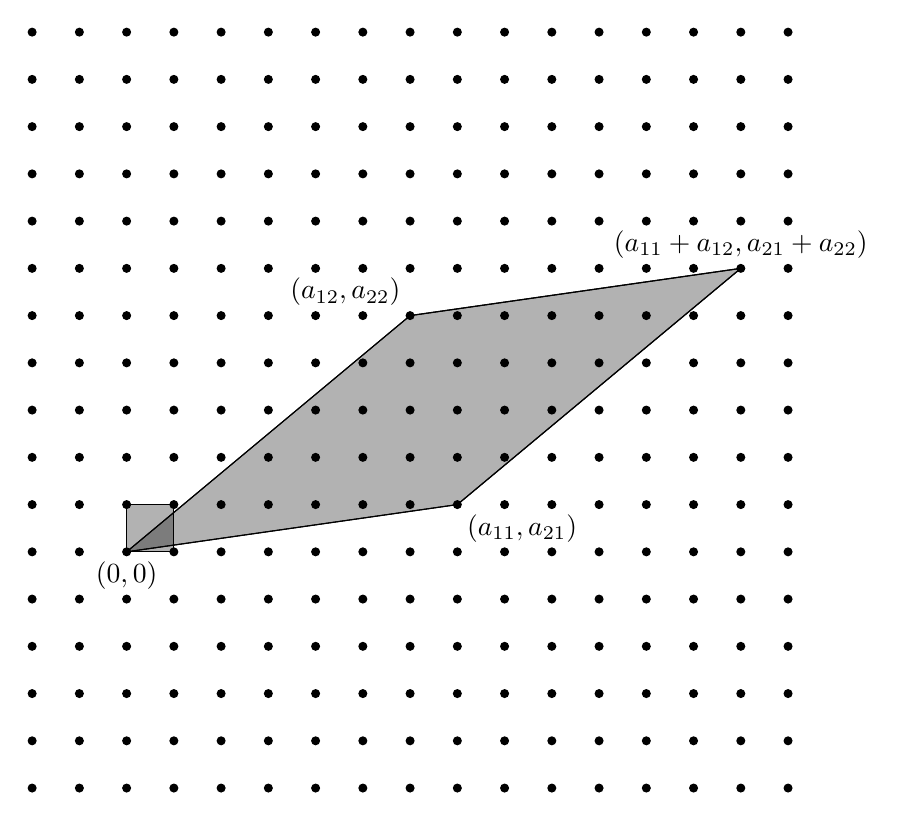
\begin{tikzpicture}[scale=0.6]

  \path (-6,-3) coordinate (O);

	\foreach \x in {-8,...,8}{% Two indices running over each
      \foreach \y in {-8,...,8}{% node on the grid we have drawn
        \node[draw,circle,inner sep=1pt,fill] at (\x,\y) {};}}

	\filldraw[fill=black, fill opacity=0.3, draw=black] (O) rectangle +(1,1);

	\draw (O) node [below] {$(0,0)$} -- +(7,1) node [below right] {$(a_{11},a_{21})$} -- +(13,6) node [above] {$(a_{11}+a_{12},a_{21}+a_{22})$} -- +(6,5) node [above left] {$(a_{12},a_{22})$} -- cycle;

	\filldraw[fill=black, fill opacity=0.3] (O) -- +(7,1) -- +(13,6) -- +(6,5) -- cycle;

  \end{tikzpicture}
  \caption{O quadrado $[0,1]^2$ e o paralelogramo $T([0,1]^2)$}
\end{figure}

\end{comment}
%%%%%%%%%%%%%%%%%%%%%%%%%%%%%%%%%%%%%%%%%%%%%
%%%%%%%%%%%%%%%%%%%COMENTÁRIO%%%%%%%%%%%%%%%%%%%
%%%%%%%%%%%%%%%%%%%%%%%%%%%%%%%%%%%%%%%%%%%%%


